\documentclass[aps,pra,twocolumn,superscriptaddress,nofootinbib]{revtex4-2}
\usepackage{amsmath,amssymb,amsthm}
\usepackage{graphicx}
\usepackage{booktabs}
\usepackage{tikz}
\usetikzlibrary{positioning,arrows.meta,shapes.misc}
\usepackage[colorlinks=true,linkcolor=blue!50!black,citecolor=blue!50!black,urlcolor=blue!50!black]{hyperref}

\newtheorem{theorem}{Theorem}
\newtheorem{lemma}{Lemma}
% generated by sbpipe_study/make_figures.py -- do not edit
\newcommand{\dmrgEzeroErr}{2.3\times10^{-11}}
\newcommand{\dmrgEoneErr}{2.4\times10^{-11}}
\newcommand{\dmrgGammaErr}{4.0\times10^{-8}}
\newcommand{\weylErr}{1.2\times10^{-14}}
\newcommand{\nSim}{96}
\newcommand{\nSimOK}{96}
\newcommand{\nPlans}{144}
\newcommand{\boundRatioMin}{2.4}
\newcommand{\boundRatioMax}{4.0\times10^{5}}
\newcommand{\boundRatioMed}{14}
\newcommand{\leakRatioMin}{1.1}
\newcommand{\leakRatioMax}{1.3\times10^{5}}
\newcommand{\leakRatioMed}{4.3}
\newcommand{\trotRatioMin}{26}
\newcommand{\trotRatioMax}{4.5\times10^{3}}
\newcommand{\trotRatioMed}{185}
\newcommand{\psuccRatioMin}{1.00}
\newcommand{\psuccRatioMax}{1.00}
\newcommand{\nScaleFail}{14}
\newcommand{\nScale}{144}
\newcommand{\fitAOptTwoCnot}{6.1}
\newcommand{\fitAOptTwoSteps}{4.3}
\newcommand{\fitAOptOneCnot}{8.0}
\newcommand{\fitAOptOneSteps}{6.2}
\newcommand{\fitADyaTwoCnot}{4.9}
\newcommand{\fitADyaTwoSteps}{2.6}
\newcommand{\fitADyaOneCnot}{6.2}
\newcommand{\fitADyaOneSteps}{4.0}
\newcommand{\fitBOptTwoCnot}{6.3}
\newcommand{\fitBOptTwoSteps}{4.6}
\newcommand{\fitBOptOneCnot}{8.4}
\newcommand{\fitBOptOneSteps}{6.7}
\newcommand{\fitBDyaTwoCnot}{5.0}
\newcommand{\fitBDyaTwoSteps}{2.7}
\newcommand{\fitBDyaOneCnot}{6.5}
\newcommand{\fitBDyaOneSteps}{4.2}
\newcommand{\fitCOptTwoCnot}{4.9}
\newcommand{\fitCOptTwoSteps}{3.7}
\newcommand{\fitCOptOneCnot}{6.5}
\newcommand{\fitCOptOneSteps}{5.3}
\newcommand{\fitCDyaTwoCnot}{3.5}
\newcommand{\fitCDyaTwoSteps}{2.1}
\newcommand{\fitCDyaOneCnot}{4.6}
\newcommand{\fitCDyaOneSteps}{3.3}
\newcommand{\cnotFortyEight}{$5.4\times10^{8}$}
\newcommand{\tFortyEight}{$1.3\times10^{10}$}
\newcommand{\schedFortyEight}{dyadic}
\newcommand{\gainOrderMin}{16}
\newcommand{\gainOrderMax}{661}
\newcommand{\gainOrderMed}{92}
\newcommand{\gainOptMin}{0.7}
\newcommand{\gainOptMax}{3.7}
\newcommand{\gainOptMed}{2.9}
\newcommand{\nDyaWins}{1}
\newcommand{\nOptCmp}{29}
\newcommand{\qetuFail}{0}
\newcommand{\qetuN}{36}
\newcommand{\qetuDyaMed}{3.3}
\newcommand{\qetuDyaMin}{2.1}
\newcommand{\qetuDyaMax}{3.9}
\newcommand{\qetuOptMed}{1.00}
\newcommand{\qetuOptMin}{0.85}
\newcommand{\qetuOptMax}{4.3}
\newcommand{\qetuOptN}{29}
\newcommand{\qetuBestMed}{1.09}
\newcommand{\qetuFortyEight}{$1.6\times10^{8}$}
\newcommand{\qetuNSim}{24}
\newcommand{\qetuNSimOK}{24}
\newcommand{\qetuBoundMed}{7.5}
\newcommand{\qetuLeakMed}{1.3}
\newcommand{\drvGapExp}{1.50}
\newcommand{\drvGapExpMin}{1.44}
\newcommand{\drvGapExpMax}{1.60}
\newcommand{\drvGamExp}{1.13}
\newcommand{\drvGamExpMin}{1.03}
\newcommand{\drvGamExpMax}{1.19}
\newcommand{\drvGamRaw}{1.52}
\newcommand{\drvNExp}{1.6}
\newcommand{\drvNExpMin}{1.4}
\newcommand{\drvNExpMax}{1.8}
\newcommand{\drvValN}{120}
\newcommand{\drvValOk}{120}
\newcommand{\drvValMed}{0.06}
\newcommand{\drvValMax}{0.43}
\newcommand{\drvValNmax}{14}
\newcommand{\drvNPlans}{3328}
\newcommand{\drvGamSpread}{2\times10^{3}}
\newcommand{\empN}{675}
\newcommand{\empKone}{675}
\newcommand{\empDegRatio}{1.09}
\newcommand{\empDegRatioMax}{6.0}
\newcommand{\empCertRatio}{23}
\newcommand{\empCertRatioMin}{7}
\newcommand{\empCertRatioMax}{2\times10^{2}}
\newcommand{\empCertK}{16}
\newcommand{\empGamRaw}{1.21}
\newcommand{\empGamLog}{0.97}
\newcommand{\empGamCert}{1.45}
\newcommand{\empGapExp}{0.98}
\newcommand{\empGapDeg}{1.00}
\newcommand{\empGapCert}{1.38}
\newcommand{\empNMatch}{2.3}
\newcommand{\empNMatchCert}{2.0}
\newcommand{\empNMatchDeg}{1.1}
\newcommand{\empNFixed}{3.1}
\newcommand{\empNFixedCert}{3.1}
\newcommand{\empNFixedDeg}{1.9}
\newcommand{\empMatchJ}{0.384, 0.510, 0.539, 0.550, 0.555}
\newcommand{\regDirect}{53}
\newcommand{\regNone}{4}
\newcommand{\regTotal}{57}
\newcommand{\cylGamSixteen}{0.91}
\newcommand{\cylGamSixtyfour}{0.9994}
\newcommand{\actWins}{26}
\newcommand{\actRatioMax}{6.3}
\newcommand{\actRatioLo}{1.0}
\newcommand{\goMDa}{10.3}
\newcommand{\goMDN}{1.42}
\newcommand{\goMDgap}{1.36}
\newcommand{\goMDL}{1.71}
\newcommand{\goMDrms}{1.26}
\newcommand{\goMDmax}{2.1}
\newcommand{\goMDgam}{0.74}
\newcommand{\goMOa}{8.08}
\newcommand{\goMON}{1.45}
\newcommand{\goMOgap}{1.58}
\newcommand{\goMOL}{1.58}
\newcommand{\goMOrms}{1.34}
\newcommand{\goMOmax}{2.6}
\newcommand{\goMOgam}{0.79}
\newcommand{\goMQa}{16.1}
\newcommand{\goMQN}{2.13}
\newcommand{\goMQgap}{0.83}
\newcommand{\goMQL}{0.78}
\newcommand{\goMQrms}{1.04}
\newcommand{\goMQmax}{1.2}
\newcommand{\goMQgam}{0.99}
\newcommand{\goCDa}{33.8}
\newcommand{\goCDN}{2.03}
\newcommand{\goCDgap}{1.27}
\newcommand{\goCDL}{2.44}
\newcommand{\goCDrms}{1.22}
\newcommand{\goCDmax}{2.2}
\newcommand{\goCDgam}{0.98}
\newcommand{\goCOa}{3.9}
\newcommand{\goCON}{2.23}
\newcommand{\goCOgap}{1.32}
\newcommand{\goCOL}{2.79}
\newcommand{\goCOrms}{1.44}
\newcommand{\goCOmax}{3.1}
\newcommand{\goCOgam}{0.97}
\newcommand{\goCQa}{20.1}
\newcommand{\goCQN}{1.98}
\newcommand{\goCQgap}{1.12}
\newcommand{\goCQL}{2.20}
\newcommand{\goCQrms}{1.22}
\newcommand{\goCQmax}{1.9}
\newcommand{\goCQgam}{0.98}
\newcommand{\goCertRatioMed}{75}
\newcommand{\goCertRatioMin}{19}
\newcommand{\goCertRatioMax}{290}
\newcommand{\goNcases}{222}
\newcommand{\goQetuOverDyMed}{1.31}
\newcommand{\fAMDcnot}{1.2--3.0}
\newcommand{\fBMDcnot}{2.7--4.4}
\newcommand{\fAMDtime}{1.5--3.0}
\newcommand{\fBMDtime}{1.5--2.8}
\newcommand{\fAMQcnot}{1.5--2.9}
\newcommand{\fBMQcnot}{1.7--1.9}
\newcommand{\fAMQtime}{1.5--2.9}
\newcommand{\fBMQtime}{1.8--2.1}
\newcommand{\fACDcnot}{4.6--9.4}
\newcommand{\fBCDcnot}{2.2--2.6}
\newcommand{\fACDtime}{1.5--3.0}
\newcommand{\fBCDtime}{1.7--2.3}
\newcommand{\fACQcnot}{4.2--7.1}
\newcommand{\fBCQcnot}{2.0--2.1}
\newcommand{\fACQtime}{1.5--2.5}
\newcommand{\fBCQtime}{1.8--2.0}
\newcommand{\fCMDtime}{2.0}
\newcommand{\fCMDtimeLo}{1.2}
\newcommand{\fCMDtimeHi}{3}
\newcommand{\fCMDsteps}{89.4}
\newcommand{\fCMDstepsLo}{26.2}
\newcommand{\fCMDstepsHi}{339}
\newcommand{\fCMQtime}{1.3}
\newcommand{\fCMQtimeLo}{1.0}
\newcommand{\fCMQtimeHi}{2}
\newcommand{\fCMQsteps}{19.2}
\newcommand{\fCMQstepsLo}{7.3}
\newcommand{\fCMQstepsHi}{68}
\newcommand{\fQDtime}{0.65}
\newcommand{\fQDsteps}{1.40}
\newcommand{\fRzCnot}{0.25}
\newcommand{\fCps}{41}
\newcommand{\fDtDTwo}{1.25}
\newcommand{\fDtCTwo}{0.017}
\newcommand{\fDtDThree}{0.56}
\newcommand{\fDtCThree}{0.009}
\newcommand{\fDtDFour}{0.30}
\newcommand{\fDtCFour}{0.005}
\newcommand{\fitMDTN}{-0.24}
\newcommand{\fitMDTgap}{1.19}
\newcommand{\fitMDTL}{0.77}
\newcommand{\fitMDTeps}{0.04}
\newcommand{\fitMDSN}{0.08}
\newcommand{\fitMDSgap}{1.90}
\newcommand{\fitMDSL}{0.71}
\newcommand{\fitMDSeps}{0.27}
\newcommand{\fitMDCN}{1.27}
\newcommand{\fitMDCgap}{1.90}
\newcommand{\fitMDCL}{0.71}
\newcommand{\fitMDCeps}{0.26}
\newcommand{\fitMQTN}{-0.10}
\newcommand{\fitMQTgap}{1.10}
\newcommand{\fitMQTL}{0.86}
\newcommand{\fitMQTeps}{0.01}
\newcommand{\fitMQSN}{1.02}
\newcommand{\fitMQSgap}{0.96}
\newcommand{\fitMQSL}{0.86}
\newcommand{\fitMQSeps}{0.01}
\newcommand{\fitMQCN}{2.20}
\newcommand{\fitMQCgap}{0.96}
\newcommand{\fitMQCL}{0.86}
\newcommand{\fitMQCeps}{0.01}
\newcommand{\fitCDTN}{0.04}
\newcommand{\fitCDTgap}{1.10}
\newcommand{\fitCDTL}{0.84}
\newcommand{\fitCDTeps}{0.01}
\newcommand{\fitCDSN}{0.85}
\newcommand{\fitCDSgap}{1.30}
\newcommand{\fitCDSL}{2.03}
\newcommand{\fitCDSeps}{0.12}
\newcommand{\fitCDCN}{2.04}
\newcommand{\fitCDCgap}{1.30}
\newcommand{\fitCDCL}{2.03}
\newcommand{\fitCDCeps}{0.12}
\newcommand{\fitCQTN}{0.01}
\newcommand{\fitCQTgap}{1.00}
\newcommand{\fitCQTL}{0.73}
\newcommand{\fitCQTeps}{0.01}
\newcommand{\fitCQSN}{0.81}
\newcommand{\fitCQSgap}{1.14}
\newcommand{\fitCQSL}{1.84}
\newcommand{\fitCQSeps}{0.12}
\newcommand{\fitCQCN}{2.00}
\newcommand{\fitCQCgap}{1.14}
\newcommand{\fitCQCL}{1.84}
\newcommand{\fitCQCeps}{0.12}
\newcommand{\optRetried}{21}
\newcommand{\optCertRetried}{10}
\newcommand{\optPoints}{286}
\newcommand{\odMMed}{0.84}
\newcommand{\odMLo}{0.53}
\newcommand{\odMHi}{1.60}
\newcommand{\odMWins}{180}
\newcommand{\odCMed}{0.35}
\newcommand{\odCLo}{0.27}
\newcommand{\odCHi}{1.05}
\newcommand{\odCWins}{221}
\newcommand{\optPgLo}{0.52}
\newcommand{\optPgMed}{0.88}
\newcommand{\bestDyTwo}{19}
\newcommand{\bestOpTwo}{55}
\newcommand{\bestQeTwo}{0}
\newcommand{\bestDyThree}{10}
\newcommand{\bestOpThree}{63}
\newcommand{\bestQeThree}{1}
\newcommand{\bestDyFour}{4}
\newcommand{\bestOpFour}{33}
\newcommand{\bestQeFour}{37}
\newcommand{\odShotTime}{0.58}
\newcommand{\odShotSteps}{0.62}
\newcommand{\odShotCnot}{0.63}
\newcommand{\fDtOFour}{0.30}
\newcommand{\fDtOTwo}{1.24}
\newcommand{\fitMOTN}{0.13}
\newcommand{\fitMOTgap}{1.21}
\newcommand{\fitMOTL}{1.19}
\newcommand{\fitMOTeps}{0.03}
\newcommand{\fitMOSN}{0.29}
\newcommand{\fitMOSgap}{1.84}
\newcommand{\fitMOSL}{1.05}
\newcommand{\fitMOSeps}{0.24}
\newcommand{\fitMOCN}{1.47}
\newcommand{\fitMOCgap}{1.84}
\newcommand{\fitMOCL}{1.05}
\newcommand{\fitMOCeps}{0.24}
\newcommand{\fitCOTN}{0.23}
\newcommand{\fitCOTgap}{1.24}
\newcommand{\fitCOTL}{1.02}
\newcommand{\fitCOTeps}{0.03}
\newcommand{\fitCOSN}{1.13}
\newcommand{\fitCOSgap}{1.46}
\newcommand{\fitCOSL}{2.39}
\newcommand{\fitCOSeps}{0.17}
\newcommand{\fitCOCN}{2.32}
\newcommand{\fitCOCgap}{1.46}
\newcommand{\fitCOCL}{2.39}
\newcommand{\fitCOCeps}{0.17}
\newcommand{\fCMOtime}{1.3}
\newcommand{\fCMOsteps}{39}
\newcommand{\goCertRatioOptMed}{35}
\newcommand{\goCertRatioOptMin}{7}
\newcommand{\goCertRatioOptMax}{198}
\newcommand{\goQetuWinsTwo}{0}
\newcommand{\goCasesTwo}{74}
\newcommand{\goQetuWinsThree}{9}
\newcommand{\goCasesThree}{74}
\newcommand{\goQetuWinsFour}{56}
\newcommand{\goCasesFour}{74}
\newcommand{\sensGapOneMiss}{0}
\newcommand{\sensGapOneTenMiss}{2}
\newcommand{\sensGapOneQuarterMiss}{10}
\newcommand{\sensGapOneHalfMiss}{16}
\newcommand{\sensGapN}{36}
\newcommand{\sensGapOneTenWorst}{$1.1\times10^{-2}$}
\newcommand{\sensDyaQuarterMiss}{0}
\newcommand{\sensGammaMiss}{12}
\newcommand{\sensGammaN}{72}
\newcommand{\sensGammaNoFilter}{12}
\newcommand{\gapFailFactor}{1.5}
\newcommand{\gapMarginCost}{2.9}
\newcommand{\gapMarginF}{0.5}
\newcommand{\gapWorstInf}{$5.1\times10^{-2}$}
\newcommand{\gapWorstF}{3}
\newcommand{\nGapFail}{3}
\newcommand{\eZeroHiCost}{13.5}
\newcommand{\eZeroHiF}{0.1}
\newcommand{\nEzeroFail}{0}
\newcommand{\nGammaFail}{0}
\newcommand{\gammaLowCost}{9.2}
\newcommand{\nAnsatzFail}{0}
\newcommand{\bestChiList}{4, 8}
\newcommand{\nNoFilter}{12}
\newcommand{\nNoFilterChiEight}{9}
\newcommand{\nChiEight}{9}
\newcommand{\cnotFortyEightChiFour}{$9.7\times10^{6}$}
\newcommand{\tFortyEightChiFour}{$2.1\times10^{8}$}
\newcommand{\cnotFortyEightChiEight}{4{,}500}
\newcommand{\gammaFortyEightChiEight}{0.9946}
\newcommand{\oracleMin}{8.7}
\newcommand{\oracleMax}{39}
\newcommand{\oracleMed}{21}


\newcommand{\ket}[1]{|#1\rangle}
\newcommand{\bra}[1]{\langle#1|}
\newcommand{\norm}[1]{\lVert#1\rVert}

\begin{document}

\title{Scaling of matrix-product-state plus cosine-filter ground-state preparation:\\
gap, overlap and target in the $J_1$--$J_2$ model, with a comparison to QETU}

\author{Authors to be added}
\date{\today}

\begin{abstract}
A common route to a ground state on a quantum computer compiles a classical trial state and removes its
residual excited weight with a quantum filter. We study how the cost of this workflow scales, with a matrix-product
state (MPS) as the trial and the one-ancilla cosine filter of Stetcu, Baroni and Carlson (SBC) as the refinement,
on the spin-$\tfrac12$ $J_1$--$J_2$ model. A modular pipeline turns DMRG inputs into a Trotterized circuit with an
input-conditional bound on the infidelity and a gate count; the bound held in all \nSimOK{} simulated circuits.
Each controlled Heisenberg bond compiles exactly into 6 CNOTs, half the per-term count. We report two costs
throughout: \emph{certified}, the circuit the pipeline plans from the bound, which can be run as is, and
\emph{measured}, the cheapest circuit that reaches the target in exact simulation, whose filter length and Trotter
step are tuned with knowledge of the ground state and are therefore a lower reference, not a recipe. Holding the
spectral gap fixed across size by tuning $J_2$ and the trial overlap fixed by a sublattice rotation
(\goNcases{} cases, $N=8$--14, $\epsilon=10^{-2}$--$10^{-4}$), the cost factorizes into filter length, Trotter step
and gates per step. The gap sets the circuit: the evolution time follows
$T\propto\Delta^{-1}\ln[(1-\gamma)/(\gamma\epsilon)]$ independently of $N$. The overlap sets the repetitions:
lowering it thirtyfold raises the measured CNOTs per shot only \fAMDcnot$\times$, but the cost per success by a
further $1/\gamma$. Certification sizes the filter to within \fCMDtime$\times$ but asks for Trotter steps 60--75
times finer than needed. This overhead decides the comparisons. Measured, the SBC filters beat a Chebyshev
(QETU) filter at $\epsilon\ge10^{-3}$, because their long pulses tolerate Trotter steps of order $1/J_1$;
certified, QETU is cheaper than the closed-form SBC schedule in every case and is the cheapest filter in
\cQetuBestTot{} of \goNcases. Measured end to end, filtering a cheap MPS beats compiling a better one on chains
only as a last-mile polisher (\actOneWins{} of \actOneTot{} targets), but on $4\times3$ and $4\times4$ cylinders at
27 of 28 targets, by up to \actRatioMax$\times$, and still at \robLbTwo{} of 28 with MPS circuits costed at the
isometry lower bound. Certified, the filtered route wins essentially only where no MPS with $\chi\le64$ reaches the target (QETU
adds one finite win, by $1.2\times$); closing that gap needs tighter, state-dependent Trotter error bounds rather than better filters.
\end{abstract}

\maketitle

%=====================================================================================================
\section{Introduction}

A common route to a ground state on a quantum computer starts classically: an approximate method
produces a trial state that can be compiled into a short circuit, and a quantum subroutine removes its
residual excited-state weight. For one-dimensional systems the natural classical engine is
DMRG~\cite{White1992,Schollwock2011}, which yields the ground-state energy $E_0$, the gap and a
matrix-product state (MPS) whose low-bond-dimension truncations compile exactly into staircase
circuits~\cite{Ran2020}. The quantum step can be phase estimation~\cite{Ge2019}, a polynomial filter
implemented by quantum singular-value transformation~\cite{Lin2020,Gilyen2019,Dong2022}, or a product of
cosine filters implemented with a single ancilla~\cite{Stetcu2023,Choi2021}. The last option, the projection
algorithm of Stetcu, Baroni and Carlson (SBC)~\cite{Stetcu2023}, needs little beyond time evolution: each
pulse is one controlled time evolution between ancilla rotations and a measurement, the filter is designed
classically, and the success probability is known in advance.

This paper asks three questions about the SBC filter on a concrete, physically relevant model, the open
$J_1$--$J_2$ Heisenberg chain:
\begin{enumerate}
\item \emph{What does it cost?} Two-qubit gates, arbitrary rotations, evolution time and repetitions, both as
certified by an a-priori bound and as measured by exact simulation of the Trotterized circuit.
\item \emph{What sets the cost?} The spectral gap $\Delta$ and the trial overlap $\gamma$ normally change
together with system size $N$ and with the coupling. We decouple them: the gap is held fixed across $N$
by tuning $J_2$, and the overlap is held fixed by a one-parameter rotation of the trial circuit, so each can
be varied while the other stays put.
\item \emph{When does it pay off?} The alternative to filtering a cheap trial state is compiling a better
one. We compare the two routes at equal target infidelity $\epsilon$.
\end{enumerate}

The answers rest on a modular pipeline (Sec.~\ref{sec:pipeline}) that takes energy estimates and an ansatz
for any Pauli-sum Hamiltonian, designs a cosine filter with a certified suppression ratio, chooses Trotter
step counts from commutator bounds, and returns an a-priori bound on the infidelity together with a gate
count. Section~\ref{sec:application} introduces the model and validates the bound. Section~\ref{sec:gapov}
is the core of the paper: the controlled gap/overlap study, which yields the cost laws and explains them
through a factorization into filter length, Trotter step and gates per step. Section~\ref{sec:regime}
follows the natural chains to $N=48$, tests robustness to wrong inputs and measures where the filter beats
a compiled MPS. Section~\ref{sec:twod} repeats that comparison on $4\times L_x$ cylinders, where it comes out
the other way, and Sec.~\ref{sec:qetu} compares with a Chebyshev polynomial filter (QETU)~\cite{Dong2022}
under identical accounting. Section~\ref{sec:meascert} sets every measured comparison beside its certified,
implementable counterpart.

\emph{Relation to prior work.} The filter is SBC's~\cite{Stetcu2023}; it shares its circuit with the rodeo
algorithm~\cite{Choi2021,Qian2021}, which draws the times at random. Our closed-form ``dyadic'' schedule, a
halving ladder of times, is the one SBC and Rule \emph{et al.} use for quantum-number
projection~\cite{Stetcu2023,Rule2024}, and for energy it is a finite form of the rodeo
super-iteration of Cohen and Oh~\cite{CohenOh2023}, recently generalized to other geometric
ratios~\cite{Patkowski2026}; what we add is its certified bound on the scaled spectral window and its measured
cost. The optimized schedule is SBC's energy recipe with a certified constraint. The Trotter bounds are those
of Childs \emph{et al.}~\cite{Childs2021}, and the certificate follows the standard argument for polynomial
filters~\cite{Lin2020,Dong2022}. QETU has been costed with Trotterized evolution for lattice gauge
theories~\cite{Kane2023} and run on small Hubbard models~\cite{Muller2024,Karacan2024}. Resource studies that
compile an MPS or other classical trial and then refine it exist for quantum
chemistry~\cite{Fomichev2024,Berry2025,Lee2025}, and Watanabe \emph{et al.}~\cite{Watanabe2026} stop an MPS
encoder early and finish with probabilistic imaginary-time evolution on Heisenberg chains. For the
two-dimensional $J_1$--$J_2$ model, the quantum--classical crossover has been estimated for phase estimation
against DMRG with state preparation taken as negligible~\cite{Yoshioka2024}. What is new here is (i) a
controlled separation of gap and overlap at fixed size, (ii) a measured, not only bounded, account of every
resource and its factorization, which shows where the certificate's overhead sits, (iii) a like-for-like
measured comparison of cosine and Chebyshev filters, and (iv) a measured map of where filtering a cheap MPS
beats compiling a better one, in one and two dimensions. The code is the \texttt{sbpipe} package, available
with all data at \url{https://github.com/aaronseymour7/FilterPipeline}; every number below is produced by
the scripts named in Appendix~\ref{app:repro}.

%=====================================================================================================
\section{The SBC filter and the resource pipeline}
\label{sec:pipeline}

\begin{figure}[t]
\centering
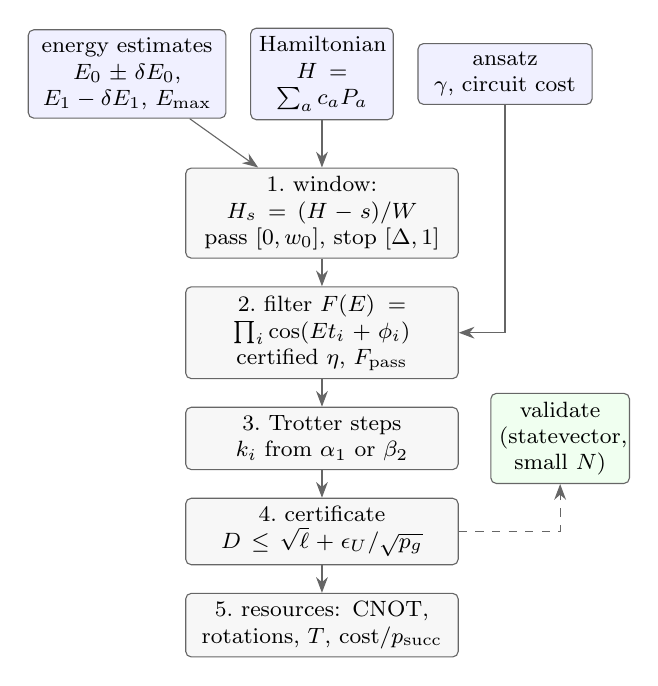
\begin{tikzpicture}[node distance=3.5mm and 3mm, font=\footnotesize,
  box/.style={draw=black!60, rounded corners=2pt, align=center, inner sep=3pt, minimum height=7mm},
  inp/.style={box, fill=blue!6}, stage/.style={box, fill=black!3, text width=3.25cm},
  arr/.style={-{Stealth[length=2mm]}, black!60}]
\node[inp, text width=2.3cm] (E) {energy estimates\\$E_0\pm\delta E_0$, $E_1-\delta E_1$, $E_{\max}$};
\node[inp, text width=1.6cm, right=of E] (H) {Hamiltonian\\$H=\sum_a c_aP_a$};
\node[inp, text width=2.0cm, right=of H] (A) {ansatz\\$\gamma$, circuit cost};
\node[stage, below=6mm of H] (W) {1.~window: $H_s=(H-s)/W$\\ pass $[0,w_0]$, stop $[\Delta,1]$};
\node[stage, below=of W] (D) {2.~filter $F(E)=\prod_i\cos(Et_i+\phi_i)$\\certified $\eta$, $F_{\rm pass}$};
\node[stage, below=of D] (T) {3.~Trotter steps $k_i$ from $\alpha_1$ or $\beta_2$};
\node[stage, below=of T] (C) {4.~certificate $D\le\sqrt{\ell}+\epsilon_U/\sqrt{p_g}$};
\node[stage, below=of C] (R) {5.~resources: CNOT, rotations, $T$, cost$/p_{\rm succ}$};
\node[box, fill=green!6, right=4mm of T, text width=1.55cm] (V) {validate\\(statevector, small $N$)};
\draw[arr] (E) -- (W); \draw[arr] (H) -- (W); \draw[arr] (A.south) |- (D.east);
\draw[arr] (W) -- (D); \draw[arr] (D) -- (T); \draw[arr] (T) -- (C); \draw[arr] (C) -- (R);
\draw[arr, dashed] (C.east) -| (V.south);
\end{tikzpicture}
\caption{The pipeline. Blue: inputs, which any classical method can supply. Grey: the stages of
\texttt{refine()}. Green: the optional statevector check used in Sec.~\ref{sec:validation}.}
\label{fig:workflow}
\end{figure}

\subsection{Inputs and the spectral window}

The Hamiltonian is $H=\sum_a c_aP_a$ with real $c_a$ and Pauli strings $P_a$, in a fixed order that is
also the Trotter order, and with an optional grouping of terms (here: one group per bond). The pipeline
assumes
\begin{equation}
\begin{gathered}
E_0\in[E_0^{\rm est}-\delta E_0,\;E_0^{\rm est}+\delta E_0],\\
E_1\ge E_1^{\rm est}-\delta E_1,\qquad E_{\rm top}\le E_{\max},
\end{gathered}
\label{eq:assumptions}
\end{equation}
where $E_1$ is the lowest level above the ground space that the trial state can overlap with. When the
trial state's quantum numbers are unknown, as for the DMRG trial states below, which are not
symmetry-adapted, this is the global first excited level; restricting to the trial state's symmetry
sector could only raise it. The certificate is a statement about the actual Hamiltonian only if
\eqref{eq:assumptions} holds for it: with an overestimated $E_1$ a real excitation can sit in the
filter's transition region, and the bound then says nothing (Sec.~\ref{sec:sens}). If no
$E_{\max}$ is given, the Weyl bound $E_{\max}=\sum_g\lambda_{\max}(h_g)$ over the term groups $h_g$ is
used; it is rigorous and, for the antiferromagnetic $J_1$--$J_2$ chain, attained by the ferromagnetic
state. With $s=E_0^{\rm est}-\delta E_0$ and $W=E_{\max}-s$, the scaled Hamiltonian $H_s=(H-s)/W$ has its
ground energy in the \emph{pass band} $[0,w_0]$, $w_0=2\delta E_0/W$, and every other relevant level in
the \emph{stop band} $[\Delta,1]$, $\Delta=(E_1^{\rm est}-\delta E_1-s)/W$.

The ansatz enters through $\gamma$, a lower estimate of its weight on the ground space, and through the
gate cost of the circuit that prepares it. A statevector is needed only for validation.

\subsection{The filter and three schedules}

One SBC pulse~\cite{Stetcu2023} applies $\mathsf H_a\,e^{-itH_s\otimes Z_a}\,R_z^{(a)}(2\phi)\,\mathsf H_a$
to the system and an ancilla in $\ket0$; the ancilla-$\ket0$ block of this unitary is
$\cos(H_st+\phi)$. (SBC write the same block with $e^{-i(tH+\delta)\otimes Y_a}$.) Keeping outcome 0
after $m$ pulses applies
\begin{equation}
F(H_s)=\prod_{i=1}^m\cos(H_st_i+\phi_i),\qquad T=\sum_i|t_i|.
\end{equation}
Two numbers characterize a filter: the pass-band floor $F_{\rm pass}\le\min_{[0,w_0]}|F|$ and the
suppression ratio $\eta=\sup_{[\Delta,1]}|F|/F_{\rm pass}$. Both are certified, not sampled: since
$|F'|\le L:=\sum_i|t_i|$ and $|F''|\le L^2$, an interval branch-and-bound gives a rigorous upper bound
on $\sup|F|$ over the stop band, and $F_{\rm pass}=|F(0)|-Lw_0$ (the certifier is
\texttt{sbpipe.floor.certify}; it is used for the optimized schedule, the other two have
closed-form certificates). Given a target leakage $\epsilon_\ell$ and $\gamma$, the
design target is $\eta^2\le\gamma\epsilon_\ell/[(1-\epsilon_\ell)(1-\gamma)]$ (Lemma~\ref{lem:leak}).
We provide three schedules:

\emph{Uniform}: $m$ equal pulses $t=\pi/(1+\Delta)$, $\phi=0$, so $F=\cos^m(Et)$. For $E\in[\Delta,1]$
we have $Et\in[\theta,\pi-\theta]$, $\theta=\pi\Delta/(1+\Delta)$, hence $\sup_{[\Delta,1]}|\cos Et|=\cos\theta$. Then
$m\approx2\ln(1/\eta)/\theta^2$ and $T\approx2\ln(1/\eta)/(\pi\Delta^2)$: quadratic in the inverse gap.
It is the baseline that any design should beat.

\emph{Dyadic}: $r$ repetitions of the halving ladder $t=\tau,2\tau,\dots,2^{K-1}\tau$,
$\tau=\pi/(1+\Delta)$, $\phi=0$. This is the schedule SBC use for quantum-number
projection~\cite{Stetcu2023,Rule2024}, and for the energy it is a finite rodeo
super-iteration~\cite{CohenOh2023} (whose infinite form gives $\sin x/x$). One block is a Dirichlet kernel,
\begin{equation}
\prod_{k=0}^{K-1}\cos(2^kE\tau)=\frac{\sin(2^KE\tau)}{2^K\sin(E\tau)},
\label{eq:dirichlet}
\end{equation}
which equals 1 at $E=0$. The identity is exact for every $E$ (repeated use of $\sin2x=2\sin x\cos x$).
The suppression bound is a separate step that uses the spectral window: for $E\in[\Delta,1]$,
$E\tau\in[\theta,\pi-\theta]$, so $\sin(E\tau)\ge\sin\theta$ and, with $|\sin(2^KE\tau)|\le1$, the block
is at most $\eta_b=1/(2^K\sin\theta)$ in absolute value there. This bound relies on the scaling $H_s$,
which places every relevant level in $[0,1]$, and on the choice of $\tau$; it does not hold outside
$[\Delta,1]$. With $r=\lceil\ln\eta/\ln\eta_b\rceil$ blocks,
$T=r\tau(2^K-1)$; choosing $2^K\sin\theta\approx e$ gives
\begin{equation}
T_{\rm dyadic}\approx\frac{e\,\tau}{\sin\theta}\ln\frac1\eta\;\approx\;\frac{e}{\Delta}\ln\frac1\eta ,
\end{equation}
the optimal $O(\Delta^{-1}\log\eta^{-1})$ scaling~\cite{Lin2020} with an explicit constant and no
optimization; Cohen and Oh reach the same conclusion for super-iterations on a generic gapped
spectrum~\cite{CohenOh2023}. The pipeline searches $K$ and $r$ for the smallest $T$. Both closed-form schedules are
certified by the inequalities just given (with $F_{\rm pass}=\cos^m(w_0t)$ and $1-Lw_0$,
respectively), which avoids interval arithmetic on filters with $L\sim10^{3}$--$10^{5}$; the
test suite checks them against a $2\times10^6$-point grid.

\emph{Optimized}: times and phases chosen to maximize $F(0)^2$ subject to the certified constraint on
$\eta$ at fixed $(T,m)$, over a grid of $x=T\Delta/\pi$ and $m\in\{4,6,8\}$, picking the pair with the
smallest $T^2/F(0)^2$. This is SBC's recipe for energy filters~\cite{Stetcu2023} with a certified
constraint in place of a grid objective; it uses the SLSQP designer \texttt{sbpipe/floor.py}.
Nonzero phases trade success probability ($F(0)<1$) for a shorter $T$.

For each schedule the leakage share $\epsilon_\ell/\epsilon\in\{0.5,0.25,0.1,0.05\}$ is scanned and the
plan with the smallest expected CNOT count per success is kept. An ``auto'' mode does the same over the dyadic and optimized
schedules together.

\subsection{Trotterization}

Each controlled evolution $e^{-it_iH_s\otimes Z_a}$ is approximated by $k_i$ steps of the first-order
(Lie) or second-order (Strang) product formula over the non-identity terms; the identity term of $H_s$
becomes a single ancilla $R_z$ per pulse and is exact. For $B_a=\sum_{b>a}H_b$ the bounds of Childs
\emph{et al.}~\cite[Props.~15--16]{Childs2021} are
\begin{align}
\norm{S_1(t)-e^{-itH}}&\le\tfrac{t^2}{2}\alpha_1,&\alpha_1&=\textstyle\sum_a\norm{[B_a,H_a]},\\
\norm{S_2(t)-e^{-itH}}&\le t^3\beta_2,&\beta_2&=\textstyle\frac1{12}\sum_a\norm{[B_a,[B_a,H_a]]}\nonumber\\
&&&\quad+\textstyle\frac1{24}\sum_a\norm{[H_a,[H_a,B_a]]},
\end{align}
so $k$ steps over time $t$ cost $\alpha_1t^2/(2k)$ or $\beta_2t^3/k^2$. The filter times $t_i$ are in
units of the scaled Hamiltonian, so the constants are evaluated for the terms of $H_s$, i.e.\ for
coefficients $c_a/W$ (the identity shift does not enter any commutator). Equivalently
$\alpha_1(H_s)=\alpha_1(H)/W^2$ and $\beta_2(H_s)=\beta_2(H)/W^3$, with physical evolution time
$t_i/W$; the code uses the first convention, and we checked that it agrees with the second to machine
precision. Tensoring every term with
$Z_a$ leaves $\alpha_1$ and $\beta_2$ unchanged because $Z_a^2=1$. For Pauli strings
$[P_b,P_a]=2P_bP_a$ when they anticommute and 0 otherwise, so each commutator is a short Pauli sum
supported on a few qubits around term $a$; we evaluate its norm exactly on that support (dense for
$\le8$ qubits, Lanczos to a relative tolerance of $10^{-12}$ up to 12 with a $10^{-9}$ safety factor,
triangle inequality beyond, which never occurred here). The Lanczos values are numerically exact but
not certified upper bounds; replacing them by the triangle inequality would make every constant
rigorous at a higher cost. The
constants are maximized over the forward and reversed term order, so they hold for either convention.
Every pulse evolves under the same $H_s\otimes Z_a$, so the per-pulse bounds
$\alpha_1t_i^2/(2k_i)$ and $\beta_2|t_i|^3/k_i^2$ share one constant; the phase $\phi_i$ enters only the
ancilla rotation, and the bound is symmetric in the sign of $t_i$. With equal constants, the continuous
relaxation of $\min\sum_ik_i$ subject to $\sum_i(\text{bound}_i)\le\epsilon_T$ is solved by
$k_i\propto|t_i|$ for both orders (Lagrange). We take $k_i=\lceil|t_i|/\delta t\rceil$ with the common
step $\delta t$ of that solution. Rounding up keeps the bound, costs at most $m$ steps more than the
continuous optimum and need not be the integer optimum; the budget it frees goes to rotation synthesis.
The certified times are untouched.

\subsection{The certificate}

\begin{theorem}\label{thm:cert}
Assume \eqref{eq:assumptions} and that the trial state has ground-space weight at least $\gamma$. Let
the designed filter have certified $\eta$ and $F_{\rm pass}$, let $\epsilon_U$ bound the operator-norm
error of the implementation (Trotter error $\sum_i\epsilon_i$ plus $R\delta$ for the $R$ arbitrary
rotations of the trial and filter circuits, each synthesized to accuracy $\delta$), and let
\begin{equation}
\ell=\frac{(1-\gamma)\eta^2}{\gamma+(1-\gamma)\eta^2},\qquad p_g=\gamma F_{\rm pass}^2 .
\end{equation}
Let $\ket g=\Pi_0\ket\psi/\norm{\Pi_0\ket\psi}$ be the normalized projection of the trial state onto
the ground space, with $\Pi_0$ the ground-space projector; $\ket g$ is a pure state also when the
ground space is degenerate. For a noiseless implementation the state $\ket{\tilde\psi_{\rm out}}$
prepared conditioned on the ancilla outcomes 0 is pure, and
\begin{equation}
D\le\sqrt\ell+\frac{\epsilon_U}{\sqrt{p_g}},\qquad
1-\operatorname{Tr}(\Pi_0\tilde\rho)\le1-|\langle g|\tilde\psi_{\rm out}\rangle|^2=D^2,
\label{eq:cert}
\end{equation}
where $D$ is the trace distance between $\tilde\rho=\ket{\tilde\psi_{\rm out}}\bra{\tilde\psi_{\rm out}}$
and $\ket g$. Moreover $\langle H\rangle-E_0\le(E_{\rm top}-E_0)D^2$, and the success probability is at
least $(\sqrt{p_g}-\epsilon_U)^2$. Below, $1-F$ denotes $1-|\langle g|\tilde\psi_{\rm out}\rangle|^2$; for
the nondegenerate ground state of the chains studied here it is the usual infidelity.
\end{theorem}

The proof (Appendix~\ref{app:proof}) combines a leakage lemma for the exact filter with the
observation that a vector error $\epsilon_U$ on an unnormalized vector of norm at least $\sqrt{p_g}$
moves its direction by at most $\epsilon_U/\sqrt{p_g}$. The pipeline sets the budget
$\epsilon_U\le(\sqrt\epsilon-\sqrt\ell)\sqrt{p_g}$, gives $90\%$ of it to the product formula and the
rest to rotation synthesis. If the trial state already satisfies $1-\gamma\le\epsilon$, the pipeline
also offers the empty filter ($\eta=1$, no post-selection, $\ell=1-\gamma$) and keeps whichever plan
is cheaper.

\subsection{Resource model}

All-to-all connectivity and the Clifford+$R_z$ gate set are assumed. Every Trotter factor of a pulse
is controlled by the ancilla. For a Heisenberg bond $(i,j)$ the three commuting terms form one exact
three-qubit block,
\begin{align}
e^{-ict(X_iX_j+Y_iY_j+Z_iZ_j)\otimes Z_a}
&=V^\dagger e^{-ict(Z_iZ_a+Z_jZ_a-Z_iZ_jZ_a)}V,\nonumber\\
V&=\mathsf H_i\,\mathrm{CNOT}_{ij},
\label{eq:bond}
\end{align}
since the Bell-basis change $V$ maps $XX,YY,ZZ$ to $Z_i,-Z_iZ_j,Z_j$. The diagonal factor is a phase
polynomial on the parities $i\oplus a$, $i\oplus j\oplus a$, $j\oplus a$, applied by
$\mathrm{CNOT}_{ia}\,R_z\,\mathrm{CNOT}_{ja}\,R_z\,\mathrm{CNOT}_{ia}\,R_z\,\mathrm{CNOT}_{ja}$ on the
ancilla wire~\cite{Amy2014}. One controlled bond thus costs 6 CNOTs and 3 $R_z$, against 12 CNOTs for three
separate weight-3 Pauli rotations and 8 for qiskit's \texttt{PauliEvolutionGate} synthesis (both checked in
the test suite, as is Eq.~\eqref{eq:bond}); it is the controlled analogue of the 3-CNOT two-qubit
gate~\cite{Vatan2004,Vidal2004}. A numerical search over 300 four-CNOT layouts found no exact circuit. The
block is the same unitary as its three term rotations, so the Trotterized circuit and its error are those of
the term-wise product formula. The cheaper control by an anticommuting Pauli string, used by
controlled-reversal rodeo circuits~\cite{BeeLindgren2025} and control-free QETU~\cite{Dong2022}, is not
available: no product of single-qubit Paulis anticommutes with all of $XX$, $YY$ and $ZZ$ on a bond. A Lie step
costs one block per bond; $k$ Strang steps cost $k(2B-2)+1$ blocks for $B$ bonds, because the two middle
half-steps and the outer half-steps of adjacent steps merge. Each pulse adds one ancilla $R_z$.
An arbitrary rotation at accuracy $\delta$ costs $3\log_2(1/\delta)$ $T$ gates, the leading term of
Ross--Selinger synthesis~\cite{Ross2016}. The cost of one attempt is the trial circuit plus the
filter, and the expected cost per success is the attempt cost divided by the certified lower bound
$(\sqrt{p_g}-\epsilon_U)^2$ on the success probability of the implemented circuit from
Theorem~\ref{thm:cert} (repeat-until-success; an early-abort protocol that measures after each pulse
would be cheaper and is not modeled). The pipeline spends the whole budget
$\epsilon_U=(\sqrt\epsilon-\sqrt\ell)\sqrt{p_g}$, so this denominator is
$p_g(1-\sqrt\epsilon+\sqrt\ell)^2\ge(1-\sqrt\epsilon)^2p_g$, i.e.\ at least $0.81\,p_g$ at
$\epsilon=10^{-2}$. Without a filter nothing is post-selected and every attempt succeeds. Alongside
each $T$ count we report the number of arbitrary rotations per attempt and their common synthesis
accuracy $\delta$.

%=====================================================================================================
\section{Model, inputs and validation}
\label{sec:application}

\subsection{Model and front end}

We study the open spin-$\frac12$ chain
\begin{equation}
H=J_1\sum_{i=1}^{N-1}\mathbf S_i\cdot\mathbf S_{i+1}+J_2\sum_{i=1}^{N-2}\mathbf S_i\cdot\mathbf S_{i+2},
\end{equation}
$J_1=1$, at $J_2=0$ (Heisenberg), $J_2=0.2411$ (close to the critical point of the
gapless-to-dimerized transition~\cite{Okamoto1992,Eggert1996}) and $J_2=0.4$ (dimerized), for $N=8$ to
48. Its Pauli form has $B=N-1$ bonds ($3B$ terms of weight 2) at $J_2=0$ and $B=2N-3$ otherwise. Terms are ordered by bond: nearest-neighbor bonds
with even then odd left site, then next-nearest-neighbor bonds likewise.

The front end (\texttt{sbpipe/frontends/dmrg\_quimb.py}) builds the MPO from the Pauli sum and runs
two-site DMRG (quimb~\cite{Gray2018}) with bond dimensions up to 256 ($N\le24$) or 128 ($N>24$) and
truncation cutoff $10^{-12}$. $E_1$ is the lowest state of $H+\mu(S^z_{\rm tot}-1)^2$, $\mu=2$, i.e.\
the lowest triplet, which we use as the global first excitation. The error bars $\delta E_0,\delta E_1$
are the energy change between the last two bond dimensions, floored at $10^{-10}$; they are
convergence heuristics, not bounds. Both DMRG energies are variational upper bounds, so a residual
DMRG error in $E_1$ (or convergence of the penalty run to a higher state) biases the gap upward, which
is the dangerous direction (Sec.~\ref{sec:sens}); these error bars do not protect against that bias, and
the certificate for $N>14$ is conditional on the gap. The trial state is
the variationally optimal MPS at fixed bond dimension $\chi\in\{1,2,4,8\}$, and $\gamma$ is its
overlap with the reference MPS. This is an estimate of the overlap with the exact ground state, not a
lower bound on it, so for $N>14$ the certificate is equally conditional on $\gamma$. An MPS of bond dimension $2^b$ is exactly a staircase of $N-b$ unitaries
on $b+1$ qubits; we cost each with the quantum Shannon decomposition bound
$\frac{23}{48}4^n-\frac32 2^n+\frac43$ CNOTs (3, 20, 100 for $n=2,3,4$)~\cite{Shende2006} and $4^n-1$
rotations.

For $N\le14$ we compare with exact diagonalization (ED). DMRG reproduces $E_0$ to $\dmrgEzeroErr$,
the first excited level of any symmetry to $\dmrgEoneErr$ (so the first excitation is the triplet in
every ED case), and the trial overlaps to
$\dmrgGammaErr$ (largest difference, for a $\chi=1$ trial). The Weyl bound equals the exact top of the spectrum to $\weylErr$.
Table~\ref{tab:inputs} lists the inputs. The trial overlap decays roughly exponentially with $N$ at
fixed $\chi$, because a fixed bond dimension captures a fixed amount of entanglement per bond while
the truncation error accumulates over $N$ bonds, so the filter has more to do at larger $N$.

\begin{table}[t]
\caption{DMRG inputs: ground energy, gap $E_1-E_0$ and trial overlap $\gamma$ of the optimal
bond-dimension-$\chi$ MPS. Source: \texttt{results/inputs.json}.}
\label{tab:inputs}
\begin{ruledtabular}
\begin{tabular}{rrrrrrrr}
$N$ & $J_2$ & $E_0$ & gap & $\gamma_{\chi=1}$ & $\gamma_{2}$ & $\gamma_4$ & $\gamma_8$\\
\midrule
8 & 0 & -3.374933 & 0.3927 & 0.134 & 0.775 & 0.999 & 1.0000 \\
12 & 0 & -5.142091 & 0.2809 & 0.060 & 0.591 & 0.994 & 1.0000 \\
16 & 0 & -6.911737 & 0.2193 & 0.028 & 0.475 & 0.984 & 0.9999 \\
24 & 0 & -10.453786 & 0.1530 & 0.006 & 0.328 & 0.954 & 0.9994 \\
32 & 0 & -13.997316 & 0.1177 & 0.001 & 0.234 & 0.913 & 0.9978 \\
48 & 0 & -21.085956 & 0.0809 & 0.000 & 0.125 & 0.817 & 0.9902 \\
8 & 0.2411 & -3.135001 & 0.3859 & 0.113 & 0.904 & 1.000 & 1.0000 \\
12 & 0.2411 & -4.738077 & 0.2720 & 0.046 & 0.806 & 1.000 & 1.0000 \\
16 & 0.2411 & -6.343316 & 0.2100 & 0.019 & 0.703 & 0.998 & 1.0000 \\
24 & 0.2411 & -9.556221 & 0.1443 & 0.003 & 0.517 & 0.989 & 0.9997 \\
32 & 0.2411 & -12.770432 & 0.1099 & 0.001 & 0.373 & 0.972 & 0.9989 \\
48 & 0.2411 & -19.200243 & 0.0744 & 0.000 & 0.191 & 0.920 & 0.9946 \\
8 & 0.4 & -3.025191 & 0.4037 & 0.036 & 0.976 & 1.000 & 1.0000 \\
12 & 0.4 & -4.545626 & 0.2956 & 0.003 & 0.945 & 1.000 & 1.0000 \\
16 & 0.4 & -6.066666 & 0.2371 & 0.000 & 0.911 & 0.999 & 1.0000 \\
24 & 0.4 & -9.109325 & 0.1748 & 0.000 & 0.839 & 0.995 & 0.9998 \\
32 & 0.4 & -12.152237 & 0.1418 & 0.000 & 0.768 & 0.990 & 0.9995 \\
48 & 0.4 & -18.238247 & 0.1075 & 0.000 & 0.640 & 0.976 & 0.9981 \\

\end{tabular}
\end{ruledtabular}
\end{table}

\subsection{Validation of the certificate ($N\le14$)}
\label{sec:validation}

For $N\in\{8,10,12,14\}$, the three couplings, $\epsilon\in\{10^{-2},10^{-3}\}$, the three schedules and
both Trotter orders we plan a circuit for the $\chi=2$ trial state and, when its size permits,
simulate it exactly: the ancilla-0 block of the Trotterized circuit is
$\frac12(e^{-i\phi}S(t)+e^{i\phi}S(-t))$ per pulse, applied to the trial statevector and compared with
the ED ground state. Of \nPlans{} plans, \nSim{} were simulated (the others, mostly uniform or first-order plans
with $10^{4}$--$10^{8}$ steps, exceed our simulation budget), and the certificate held in all
\nSimOK{} (Fig.~\ref{fig:validation}).

\begin{figure}[t]
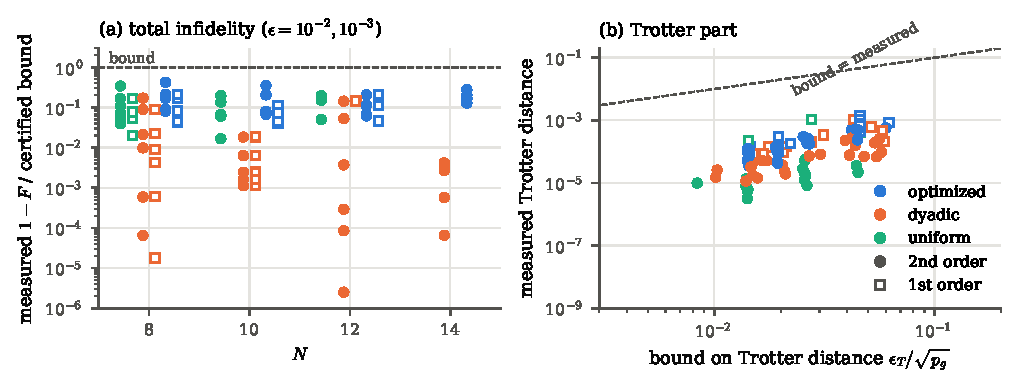
\includegraphics[width=\columnwidth]{figs/fig_validation.pdf}
\caption{All simulated plans. (a) Measured infidelity of the planned circuit divided by its certified
bound; points below the dashed line respect the bound and are offset horizontally by schedule and
order. (b) Measured distance between the Trotterized and the exact filtered state against
its certified bound. Points below the dashed lines respect the bound. Filled circles: second order;
open squares: first order.}
\label{fig:validation}
\end{figure}

The bound is conservative by a median factor \boundRatioMed{} (range \boundRatioMin--$\boundRatioMax$)
in infidelity. Splitting it shows where: the leakage term $\ell$ overestimates the exact filter's
infidelity by a median \leakRatioMed$\times$ (range \leakRatioMin--$\leakRatioMax$). By schedule the medians are 1.4 (optimized), 4 (uniform)
and 54 (dyadic): the optimized design pushes $|F|$ to $\eta F_{\rm pass}$ across the band, whereas the
closed-form dyadic bound $1/(2^K\sin\theta)$ is reached only near the band edge. More generally, $\eta$ is
a worst case over the whole stop band while the trial state's excited weight sits mostly low in the
band. The
Trotter term overestimates the measured Trotter distance by a median \trotRatioMed$\times$ (range
\trotRatioMin--$\trotRatioMax$): commutator bounds are worst-case over all states, while the filtered state lives in the low-energy
subspace, where Trotter errors are much smaller~\cite{Sahinoglu2021,Mizuta2025}, and empirical Trotter errors
are known to lie far below the bounds~\cite{Childs2018}. The measured success probability
equals $p_g$ to two digits in every case, because after filtering almost all of the surviving norm is
ground-state weight.

Table~\ref{tab:schedules} compares the schedules for one case. The uniform filter needs a total time
an order of magnitude larger than the others, as its $\Delta^{-2}$ scaling predicts. The optimized
filter is shortest; its nonzero phases lower $p_g$ (0.58 against 0.81 here), which the cost criterion
accounts for. Second order cuts the step count by one to two orders of magnitude at these sizes.
Figure~\ref{fig:filters} shows the three filter functions.

\begin{figure}[t]
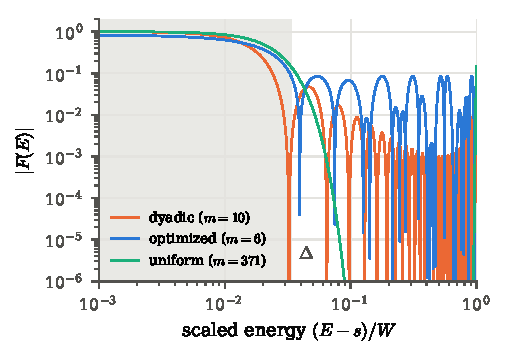
\includegraphics[width=0.95\columnwidth]{figs/fig_filters.pdf}
\caption{$|F(E)|$ of the three schedules for $N=12$, $J_2=0.2411$, $\epsilon=10^{-2}$, second order.
Dotted lines: certified $\eta F_{\rm pass}$. Grey: the gap region. The horizontal axis is linear below
$\Delta$ and logarithmic above.}
\label{fig:filters}
\end{figure}

\begin{table*}[t]
\caption{Plans for $N=12$, $J_2=0.2411$, $\chi=2$ trial. $T_{\rm phys}=T/W$ in units of $1/J_1$; CNOT and
$T$ counts per attempt (filter) and expected per success (trial + filter, divided by the certified
success probability $(\sqrt{p_g}-\epsilon_U)^2$). ``rot.'': arbitrary rotations per attempt (trial +
filter), each synthesized to accuracy $\delta$. ``meas.'': simulated infidelity of the planned circuit.
Source: \texttt{results/validate.json}.}
\label{tab:schedules}
\begin{ruledtabular}
\begin{tabular}{rlrrrrrrrrrrr}
$\epsilon$ & schedule & order & $m$ & $T_{\rm phys}$ & $p_g$ & steps & CNOT (filter) & CNOT/success & rot. & $\delta$ & $T$/success & meas.\ $1-F$\\
\midrule
$1\times10^{-2}$ & uniform & 1 & 447 & 167.9 & 0.81 & 4{,}127{,}151 & $1.0\times10^{9}$ & $1.3\times10^{9}$ & $3.5\times10^{10}$ & -- \\
$1\times10^{-2}$ & uniform & 2 & 447 & 167.9 & 0.81 & 17{,}433 & $8.6\times10^{6}$ & $1.1\times10^{7}$ & $2.3\times10^{8}$ & $6.9\times10^{-4}$ \\
$1\times10^{-2}$ & dyadic & 1 & 10 & 23.3 & 0.81 & 54{,}466 & $1.4\times10^{7}$ & $1.7\times10^{7}$ & $3.7\times10^{8}$ & -- \\
$1\times10^{-2}$ & dyadic & 2 & 10 & 23.3 & 0.81 & 742 & $3.7\times10^{5}$ & $4.6\times10^{5}$ & $8.1\times10^{6}$ & $8.9\times10^{-7}$ \\
$1\times10^{-2}$ & optimized & 1 & 6 & 8.7 & 0.58 & 13{,}384 & $3.4\times10^{6}$ & $5.8\times10^{6}$ & $1.2\times10^{8}$ & $1.1\times10^{-3}$ \\
$1\times10^{-2}$ & optimized & 2 & 6 & 8.7 & 0.58 & 226 & $1.1\times10^{5}$ & $1.9\times10^{5}$ & $3.3\times10^{6}$ & $1.1\times10^{-3}$ \\
\midrule
$1\times10^{-3}$ & uniform & 1 & 761 & 285.9 & 0.81 & 28{,}012{,}410 & $7.1\times10^{9}$ & $8.8\times10^{9}$ & $2.6\times10^{11}$ & -- \\
$1\times10^{-3}$ & uniform & 2 & 658 & 247.2 & 0.81 & 55{,}930 & $2.8\times10^{7}$ & $3.4\times10^{7}$ & $8.3\times10^{8}$ & -- \\
$1\times10^{-3}$ & dyadic & 1 & 15 & 34.9 & 0.81 & 353{,}844 & $8.9\times10^{7}$ & $1.1\times10^{8}$ & $2.8\times10^{9}$ & -- \\
$1\times10^{-3}$ & dyadic & 2 & 15 & 34.9 & 0.81 & 2{,}304 & $1.1\times10^{6}$ & $1.4\times10^{6}$ & $2.9\times10^{7}$ & $3.2\times10^{-9}$ \\
$1\times10^{-3}$ & optimized & 1 & 8 & 14.4 & 0.67 & 80{,}421 & $2.0\times10^{7}$ & $3.0\times10^{7}$ & $7.1\times10^{8}$ & -- \\
$1\times10^{-3}$ & optimized & 2 & 8 & 14.4 & 0.67 & 709 & $3.5\times10^{5}$ & $5.2\times10^{5}$ & $1.0\times10^{7}$ & $6.2\times10^{-5}$ \\

\end{tabular}
\end{ruledtabular}
\end{table*}

How much of the remaining gap could a better bound recover? For $N\le12$ we bisect a common scale
factor on the certified $k_i$ until the simulated infidelity just meets $\epsilon$. The certified step
count is \oracleMin--\oracleMax$\times$ (median \oracleMed) larger than this oracle value
(Table~\ref{tab:oracle}). The oracle uses the exact ground state and is not a usable rule; it measures
the price of certification at second order.

\begin{table}[t]
\caption{Certified over oracle step count (second order, $\chi=2$). Columns: $N=8,10,12$ for each
$J_2$. Source: \texttt{results/oracle.json}.}
\label{tab:oracle}
\begin{ruledtabular}
\begin{tabular}{llrrrrrrrrr}
 & & \multicolumn{3}{c}{$J_2=0$} & \multicolumn{3}{c}{$J_2=0.2411$} & \multicolumn{3}{c}{$J_2=0.4$}\\
$\epsilon$ & schedule & 8 & 10 & 12 & 8 & 10 & 12 & 8 & 10 & 12\\
\midrule
$1\times10^{-2}$ & dyadic & 13 & 19 & 22 & 24 & 21 & 29 & 18 & 19 & 22 \\
$1\times10^{-2}$ & optimized & 9 & 12 & 13 & 14 & 15 & 21 & 11 & 12 & 12 \\
$1\times10^{-3}$ & dyadic & 19 & 22 & 27 & 31 & 31 & 32 & 17 & 19 & 21 \\
$1\times10^{-3}$ & optimized & 12 & 17 & 21 & 24 & 22 & 27 & 14 & 16 & 17 \\

\end{tabular}
\end{ruledtabular}
\end{table}

%=====================================================================================================
\section{Gap and overlap as independent inputs}
\label{sec:gapov}

The cost of the filter depends on two physical inputs, the gap above the ground state and the trial
state's weight on it, and on two choices, the size $N$ and the target $\epsilon$. Along any natural family
of chains these move together: at fixed $J_2$ the gap closes with $N$, and at fixed bond dimension the MPS
overlap decays with $N$. Varying $J_2$ does not help, because near the dimerized point a larger gap and a
better MPS come together. We therefore construct a family in which $\Delta$ and $\gamma$ are set
independently at every $N$, and measure the filter on it.

\subsection{Construction}

\emph{Fixed gap.} For each $N\in\{8,10,12,14\}$ and target gap $g=E_1-E_0\in\{0.30,0.35,\dots,0.55\}$ we
find $J_2$ by bisection on exact diagonalization so that the singlet--triplet gap equals $g$ to $10^{-9}$.
The gap closes with $N$ at fixed $J_2$, so larger chains need larger $J_2$; pairs without a solution below
the dimerized regime are left out (no $J_2$ gives $g\le0.35$ at $N=8$ or $g=0.30$ at $N=10$). The tuned
couplings reach $J_2=0.68$, beyond the Majumdar--Ghosh point, where a singlet could in principle drop below the
triplet. For all 26 tuned $(N,J_2)$, including $N=16$, the lowest excitation in the $S^z=0$ block, which contains
a member of every multiplet, coincides with the lowest $S^z=1$ state to $10^{-7}$, so the first excitation is the
triplet and $g$ is the true gap (\texttt{results/gapov\_e1check.json}).

\emph{Fixed overlap with a real circuit.} The trial is the variational $\chi=16$ MPS, prepared by its
staircase circuit, followed by $R_y(\theta)=e^{-i\theta Y/2}$ on every even site. A uniform rotation of all
sites would leave the overlap unchanged, because the ground state is a singlet; rotating one sublattice
breaks that symmetry and lowers $\gamma$ smoothly. $\theta$ is set by bisection so that $\gamma$ hits the
target to $10^{-12}$. The trial cost is the MPS circuit plus $N/2$ single-qubit rotations at every $\gamma$,
so the trial circuit does not change along an overlap scan.

\emph{Grid and measurements.} Study A fixes $g\in\{0.40,0.50\}$ and scans
$\gamma\in\{0.03,0.1,0.3,0.5,0.7,0.9\}$; study B fixes $\gamma\in\{0.1,0.5\}$ and scans $g$ over 0.30--0.55;
both at $\epsilon\in\{10^{-2},10^{-3},10^{-4}\}$, \goNcases{} cases in all. Each case is run with both SBC
schedules, dyadic and optimized, and with QETU for comparison (Sec.~\ref{sec:qetu}), and for each we record
two costs. \emph{Measured}, dyadic: the exact filter is applied to the trial state for each ladder $(K,r)$;
for the two shortest ladders that reach $\epsilon$, the coarsest common Strang step at which the full
Trotterized circuit still reaches $\epsilon$ is found by bisection on the state vector, and the cheaper is
kept. \emph{Measured}, optimized: SBC's design (Sec.~\ref{sec:pipeline}) for the target leakage $\epsilon$ with
the true gap and overlap, then the same step search. The numerical design occasionally converges to a
filter that barely passes the ground state, $f(E_0)^2\sim10^{-3}$, and with it a success probability far
below $\gamma$; wherever $p<\gamma/2$ the design is repeated over four optimizer seeds and two design targets
($\epsilon$, $\epsilon/2$) and the cheapest passing circuit is kept (\optRetried{} of \optPoints{} points). \emph{Certified}: Theorem~\ref{thm:cert} with exact energies (error bars $10^{-9}$), the Weyl bound and
the true $\gamma$. Both are reported per shot (one run of the circuit) and per success (divided by the
success probability $p$), and, unless stated otherwise, for the filter alone, without the trial circuit.

\subsection{The gap sets the circuit, the overlap sets the repetitions}

Figures~\ref{fig:filterA} and~\ref{fig:filterB} show CNOTs, $R_z$ rotations and evolution time per shot, and
CNOTs per success, along both scans. The two inputs act on different resources.

\emph{Per shot, the overlap enters only logarithmically.} At fixed gap, lowering $\gamma$ thirtyfold (0.9 to
0.03) raises the measured CNOTs per shot of the dyadic filter by only \fAMDcnot$\times$ over all $N$ and
$\epsilon$, and its evolution time by \fAMDtime$\times$. The filter must suppress the excited weight to
$\eta^2=\gamma\epsilon/(1-\gamma)$; a worse trial raises $(1-\gamma)/\gamma$ by a factor of 290 here, which adds
only $\ln290\approx5.7$ to $L=\ln[(1-\gamma)/(\gamma\epsilon)]$, already 2--13 across these cases. The dyadic
filter grows in whole pulses, so a worse trial often needs no extra pulse at all; its per-shot cost moves in
steps (Fig.~\ref{fig:filterA}, top).

\emph{Per shot, the gap enters as a power.} At fixed overlap, closing the gap by $1.8\times$ (0.55 to 0.30)
raises the CNOTs per shot by \fBMDcnot$\times$ and the evolution time by \fBMDtime$\times$
(Fig.~\ref{fig:filterB}). The time grows about as $1/\Delta$, the cost of resolving a smaller gap.

\emph{Per success, the overlap returns as $1/\gamma$.} Every run succeeds with probability $p\approx\gamma
f(E_0)^2$, and for the dyadic filter $f(E_0)=1$, so the expected cost per success carries the factor
$1/\gamma$ (last columns of Figs.~\ref{fig:filterA} and~\ref{fig:filterB}). This is the only place where the
overlap enters as a power. The practical reading is direct: the gap decides the depth of the coherent
circuit, and with it whether the filter fits within a coherence or error budget at all; the overlap decides
how many times that circuit has to be run.

\emph{$R_z$ counts follow CNOT counts exactly.} Every controlled bond block has 3 $R_z$ and 6 CNOTs, and
each pulse adds one ancilla rotation, so $R_z/\mathrm{CNOT}=\fRzCnot$ in every case. Every statement about CNOTs below therefore holds for the
arbitrary rotations, and so for the $T$ count of a fault-tolerant implementation up to the synthesis
factor $3\log_2(1/\delta)$.

\begin{figure*}[t]
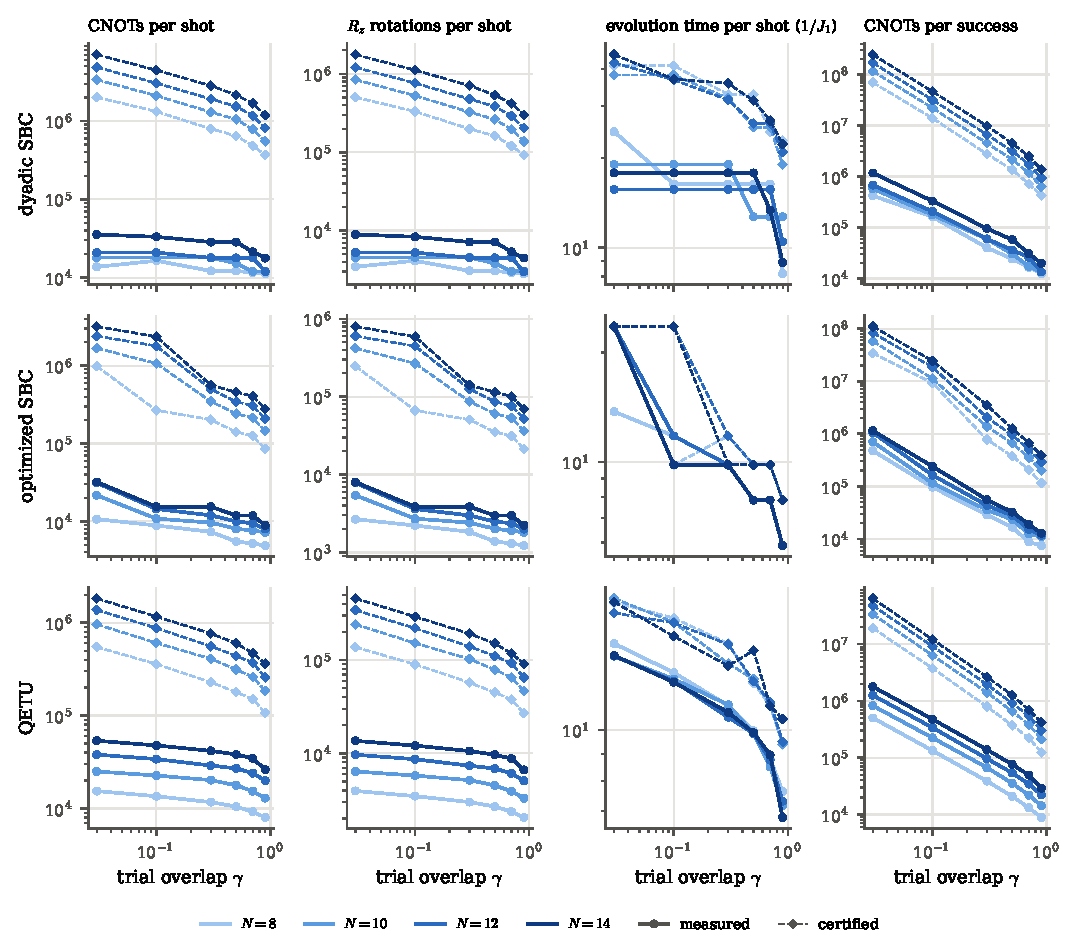
\includegraphics[width=\textwidth]{figs/fig_filter_A.pdf}
\caption{Study A: filter-only resources at a gap held at $g=0.40$ for every $N$, $\epsilon=10^{-3}$,
against the trial overlap. Rows: dyadic SBC, optimized SBC, QETU (Sec.~\ref{sec:qetu}). Solid: measured by
simulation; dashed: certified. Columns 1--3 per shot, column 4 per success. Source:
\texttt{results/gapov.jsonl}, \texttt{results/gapov\_filter.json}.}
\label{fig:filterA}
\end{figure*}

\begin{figure*}[t]
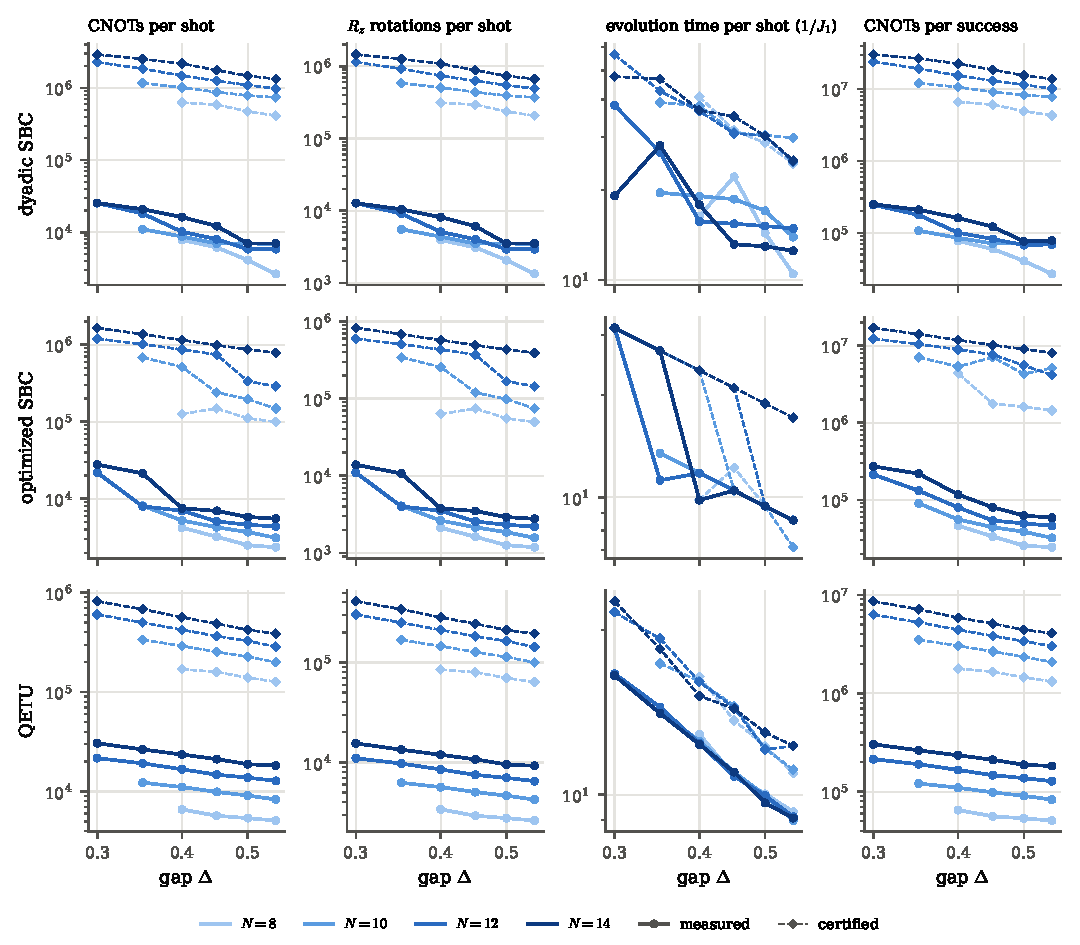
\includegraphics[width=\textwidth]{figs/fig_filter_B.pdf}
\caption{Study B: as Fig.~\ref{fig:filterA} at an overlap held at $\gamma=0.10$ for every $N$, against the gap
(held fixed across $N$ by tuning $J_2$).}
\label{fig:filterB}
\end{figure*}

\subsection{Mechanism: filter length, Trotter step and gates per step}

The per-shot cost factorizes as
\begin{equation}
\text{CNOTs per shot}=\frac{T}{\delta t}\times c_{\rm step}(N),
\label{eq:factor}
\end{equation}
and each factor answers to different inputs (Fig.~\ref{fig:mech}).

\emph{Filter length.} The physical evolution time $T$ (in $1/J_1$) depends on $\Delta$ and $L$ only. Fitting
all cases to $a\,N^{\alpha}\Delta^{-\beta}L^{\lambda}\epsilon^{-e}$, the measured dyadic filter has
$T\propto\Delta^{-\fitMDTgap}L^{\fitMDTL}$ with $N^{\fitMDTN}$, and the certified one
$T\propto\Delta^{-\fitCDTgap}L^{\fitCDTL}$ with $N^{\fitCDTN}$: at a fixed gap in absolute units, the
filter's length does not depend on the size of the system. The certified length is a median
\fCMDtime$\times$ the measured one (range \fCMDtimeLo--\fCMDtimeHi): the certificate sizes the filter
nearly right.

\emph{Trotter step.} The measured dyadic filter tolerates very coarse steps: median $\delta t=\fDtDTwo$,
\fDtDThree, \fDtDFour{} (in $1/J_1$) at $\epsilon=10^{-2}$, $10^{-3}$, $10^{-4}$, growing with the gap. Its
pulses are long and smooth, and the filtered state lives at the bottom of the spectrum, where Trotter errors
are much smaller than their worst case~\cite{Sahinoglu2021}. The certified step must cover the worst case
over the whole evolution: median $\delta t=\fDtCTwo$, \fDtCThree, \fDtCFour, about 60--75 times finer, and
shrinking as the total time grows. As a result the certified step count grows as $L^{\fitCDSL}$ against
$L^{\fitMDSL}$ measured, and is a median \fCMDsteps$\times$ (range \fCMDstepsLo--\fCMDstepsHi) the
measured one. Almost all of the certificate's overhead is in the Trotter bound, not in the filter.

\emph{Gates per step.} One Strang step costs a median $\fCps\,N$ CNOTs for the two-neighbor chain
($6(2B-2)$ with $B=2N-3$ bonds). The
measured dyadic step count barely grows with $N$ (exponent \fitMDSN), so its CNOTs grow as
$N^{\fitMDCN}$; the certified step count grows as $N^{\fitCDSN}$ through the commutator constant and the
scaled time, giving $N^{\fitCDCN}$.

\begin{figure*}[t]
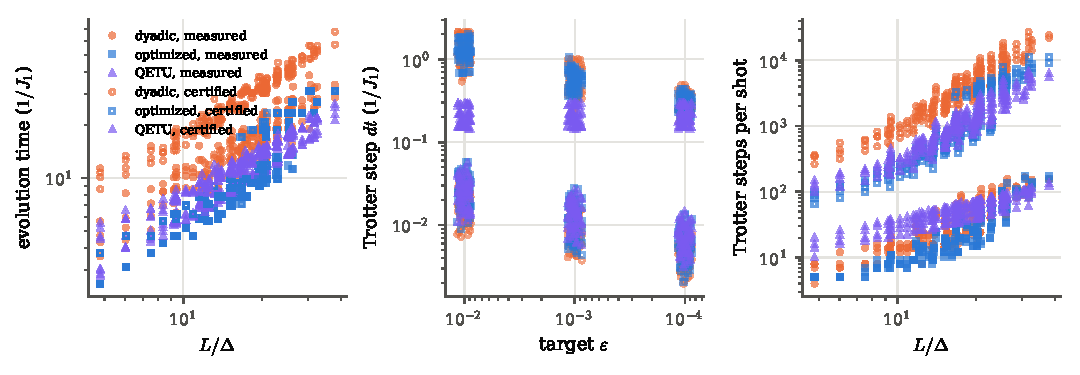
\includegraphics[width=\textwidth]{figs/fig_filter_mech.pdf}
\caption{All \goNcases{} cases. (a) Evolution time against $L/\Delta$, $L=\ln[(1-\gamma)/(\gamma\epsilon)]$.
(b) Trotter step against $\epsilon$ (jittered horizontally). (c) Trotter steps per shot against $L/\Delta$.
Filled: measured; open: certified. Orange circles: dyadic SBC; blue squares: optimized SBC; purple
triangles: QETU.}
\label{fig:mech}
\end{figure*}

\subsection{Cost laws}

Fitting the expected CNOTs per success (filter and trial circuit, as a user would pay them) to
\begin{equation}
C\approx a\,N^{\alpha}\,\Delta^{-\beta}\,L^{\lambda}\,\gamma^{-g},\qquad L=\ln\frac{1-\gamma}{\gamma\epsilon},
\label{eq:fit}
\end{equation}
over all \goNcases{} cases gives Table~\ref{tab:gofit}. For the dyadic filter,
\begin{align}
C_{\rm meas}&\approx\goMDa\,N^{\goMDN}\Delta^{-\goMDgap}L^{\goMDL}\gamma^{-\goMDgam},\\
C_{\rm cert}&\approx\goCDa\,N^{\goCDN}\Delta^{-\goCDgap}L^{\goCDL}\gamma^{-\goCDgam},
\end{align}
within a typical factor of \goMDrms{} and \goCDrms{} respectively. The certified law has the $1/\gamma$ of
the repetitions and an $L^{2.4}$ from the Trotter bound; the measured law grows more slowly in both $N$ and
$L$. The measured dyadic $\gamma$ exponent is below one because its success probability ranges from 0.76
to 1.24 times $\gamma$: at the coarse steps it tolerates, each Trotterized pulse is slightly off-diagonal in
the eigenbasis and moves weight into or out of the ground state. Part of its $\gamma$ dependence is
therefore absorbed into $L$. Across all cases the certified cost lies
\goCertRatioMin--\goCertRatioMax$\times$ (median \goCertRatioMed) above the measured one. These exponents
summarize $N=8$--14 and $g=0.30$--0.55; they describe the data and are not asymptotic laws.

\begin{table}[t]
\caption{Fits of the expected CNOTs per success to Eq.~\eqref{eq:fit} over all \goNcases{} gap/overlap
cases. ``rms''/``max'': typical and worst factor between a case and its fit. Source:
\texttt{results/gapov.jsonl}.}
\label{tab:gofit}
\begin{ruledtabular}
\begin{tabular}{lrrrrrrrr}
 & cases & $a$ & $\alpha$ & $\beta$ & $\lambda$ & $g$ & rms & max\\
\midrule
dyadic, measured & 222 & $1.0\times10^{1}$ & 1.50 & 1.15 & 1.41 & 0.78 & 1.23 & 1.9 \\
optimized, measured & 222 & $9.8$ & 1.50 & 1.36 & 1.24 & 0.83 & 1.30 & 2.3 \\
QETU, measured & 222 & $1.3\times10^{1}$ & 2.09 & 0.74 & 0.68 & 0.99 & 1.04 & 1.2 \\
dyadic, certified & 222 & $1.5\times10^{1}$ & 2.07 & 1.27 & 2.43 & 0.98 & 1.22 & 2.2 \\
optimized, certified & 222 & $1.9$ & 2.27 & 1.30 & 2.74 & 0.97 & 1.45 & 3.2 \\
QETU, certified & 222 & $9.5$ & 2.03 & 1.11 & 2.17 & 0.99 & 1.22 & 2.0 \\

\end{tabular}
\end{ruledtabular}
\end{table}

\subsection{Dyadic versus optimized SBC}
\label{sec:dyaopt}

The two SBC schedules reach the same physics by different routes. The dyadic ladder has zero phases, so it
passes the ground state with $f(E_0)=1$ and its length grows in whole pulses. The optimized design
(times and phases from SBC's recipe with a certified suppression constraint) is shorter, at the price of
$f(E_0)<1$: its measured success probability is a median \optPgMed{} times $\gamma$ (as low as
\optPgLo). Measured per shot, the optimized filter uses a median \odShotTime{} times the dyadic evolution
time and \odShotSteps{} times its Trotter steps; its tolerated step is the same, median $\delta
t=\fDtOTwo$ at $\epsilon=10^{-2}$ and \fDtOFour{} at $10^{-4}$. Per success, after the lower success
probability is paid, it is still a median \odMMed$\times$ the dyadic cost (range \odMLo--\odMHi) and the
cheaper one in \odMWins{} of \goNcases{} cases. Certified, the advantage is larger, a median \odCMed$\times$
(cheaper in \odCWins{} of \goNcases), because the optimized filter's leakage bound is nearly tight while the
closed-form dyadic bound is loose (Sec.~\ref{sec:validation}), and the shorter filter needs a looser Trotter
budget; its certified cost lies \goCertRatioOptMin--\goCertRatioOptMax$\times$ (median
\goCertRatioOptMed) above the measured one, against \goCertRatioMed$\times$ for dyadic.

Counting the cheapest of the three filters case by case, the optimized SBC filter wins \bestOpTwo{} of
\goCasesTwo{} cases at $\epsilon=10^{-2}$ (dyadic the other \bestDyTwo), \bestOpThree{} at $10^{-3}$
(dyadic \bestDyThree, QETU \bestQeThree), and \bestOpFour{} at $10^{-4}$, where QETU takes \bestQeFour{} and
dyadic \bestDyFour. The cost laws of Table~\ref{tab:gofit} make the trade-off explicit: the optimized
measured cost grows more steeply with the gap ($\Delta^{-\goMOgap}$ against $\Delta^{-\goMDgap}$), because its
design is matched to the gap, and less steeply with $L$. The price of the optimized schedule is its
design: a nonconvex optimization of about 40\,s per case that converged to a filter with $f(E_0)^2\sim10^{-3}$
in \optRetried{} of \optPoints{} measured points and had to be repeated with other seeds; the dyadic ladder
needs no design and never fails.

\subsection{Cost maps}

Two maps make the interplay visible. At fixed $N$ and $\epsilon=10^{-2}$ (Fig.~\ref{fig:gridmap}), the
contours of the dyadic cost per success run nearly parallel to the gap axis for $g\gtrsim0.40$: there the
overlap alone sets the cost, from $2$--$6\times10^3$ CNOTs at $\gamma=0.9$ to $1$--$4\times10^5$ at
$\gamma=0.03$; below $g\approx0.40$ the gap starts to matter, and $g=0.30$ costs 1.3--2.7 times $g=0.40$ at the
same overlap. The optimized filter is cheaper over most of the map, and its contours tilt toward the gap axis
over the whole range, as its steeper gap exponent implies. Per shot (not shown) the contours of both turn by
ninety degrees and the gap alone sets the circuit. At fixed gap and overlap (Fig.~\ref{fig:heat}), the
measured cost per success grows 7--21$\times$ (dyadic) from $\epsilon=10^{-2}$ to $10^{-5}$ and
1.8--4.6$\times$ from $N=8$ to 14; the contours tilt toward the $\epsilon$ axis, so over this range the target matters more
than the size. The optimized filter's lead is largest at loose targets and at $\gamma=0.5$, and shrinks
toward $\epsilon=10^{-5}$.

\begin{figure*}[t]
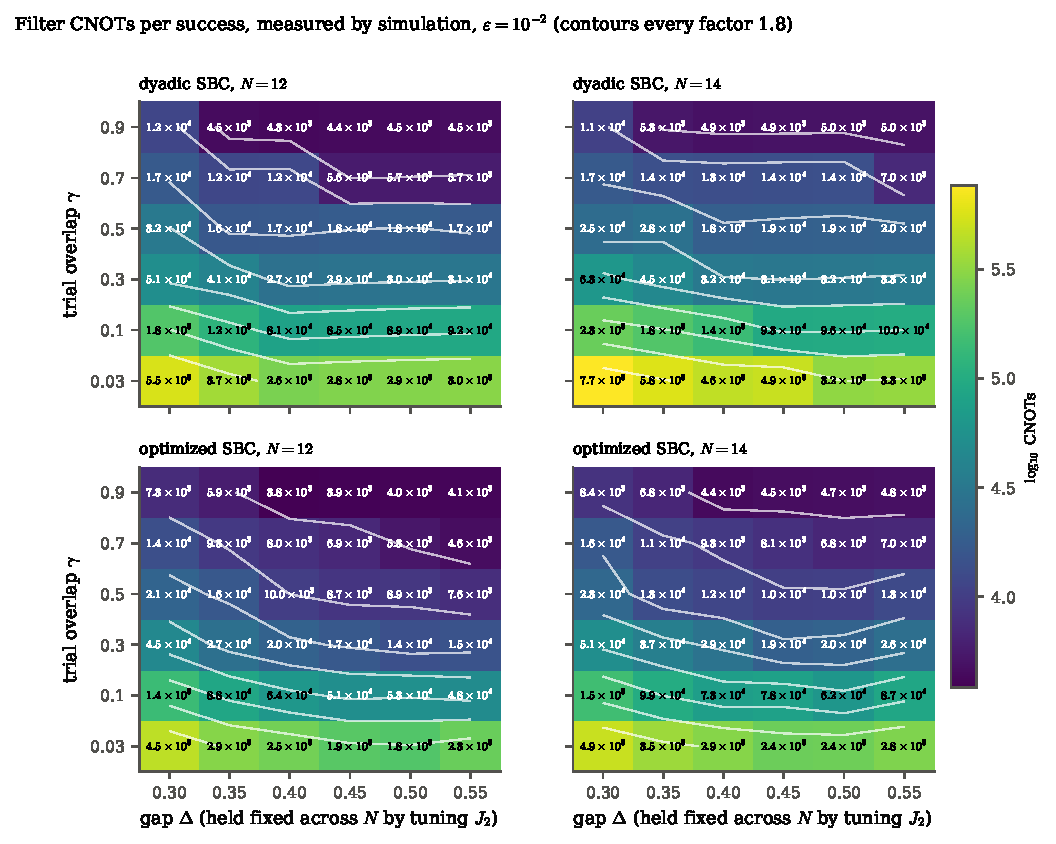
\includegraphics[width=0.85\textwidth]{figs/fig_gridmap.pdf}
\caption{Filter CNOTs per success over gap and overlap at $\epsilon=10^{-2}$, measured, for the dyadic
(top) and optimized (bottom) SBC filters at $N=12$ and 14. White contours every factor 1.8. Source:
\texttt{results/gapov.jsonl}, \texttt{results/gapov\_grid.jsonl}.}
\label{fig:gridmap}
\end{figure*}

\begin{figure*}[t]
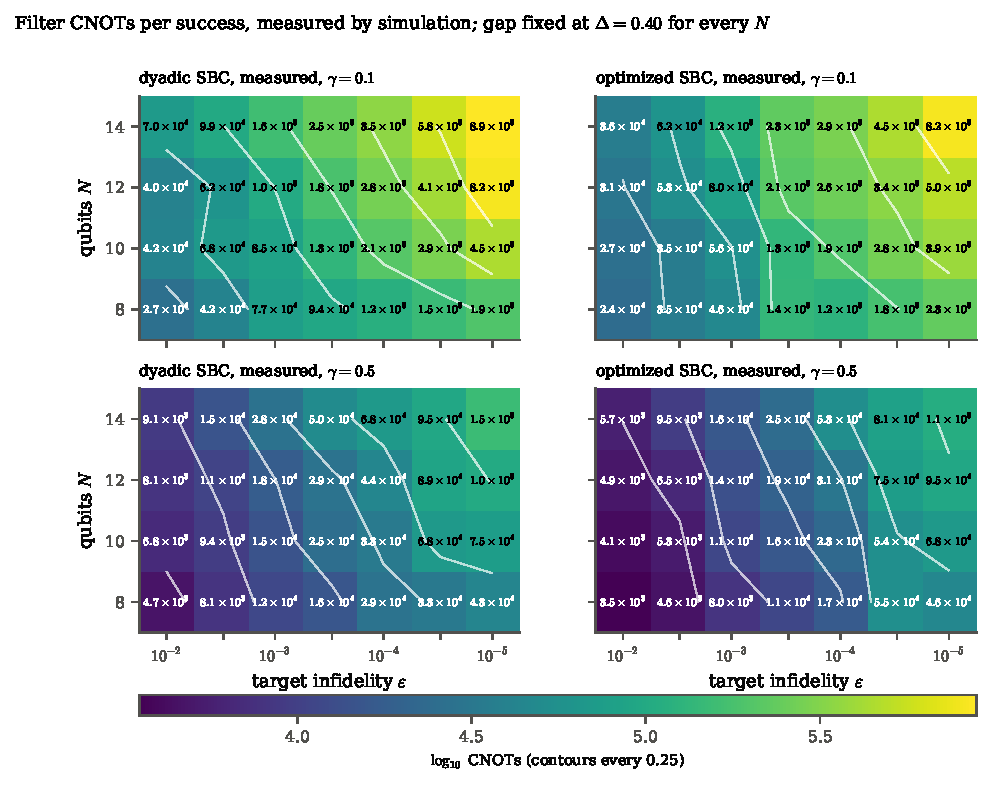
\includegraphics[width=0.85\textwidth]{figs/fig_heat_meas_succ.pdf}
\caption{Filter CNOTs per success over $N$ and $\epsilon$ at a gap held at $g=0.40$, measured, for the
dyadic (left) and optimized (right) SBC filters at $\gamma=0.1$ (top) and 0.5 (bottom). Source:
\texttt{results/gapov*.jsonl}.}
\label{fig:heat}
\end{figure*}

%=====================================================================================================
\section{Resources and regimes of advantage}
\label{sec:regime}

The controlled study fixes the inputs; here they take the values that DMRG supplies for natural chains, at
sizes beyond exact simulation, and we ask when filtering beats the alternative of compiling a better MPS.

\subsection{Resources up to $N=48$}

Without simulation the pipeline only needs DMRG, so we plan for $N$ up to 48 with the same $\chi=2$
trial family (Fig.~\ref{fig:scaling}, Table~\ref{tab:scaling}). Over all sizes, couplings and targets
the second-order plan is \gainOrderMin--\gainOrderMax$\times$ (median \gainOrderMed) cheaper than the
first-order plan of the same schedule. The optimized schedule is \gainOptMin--\gainOptMax$\times$
(median \gainOptMed) cheaper than the dyadic one at second order, and more expensive in \nDyaWins{} of
\nOptCmp{} comparable cases. Its numerical design, however, failed in \nScaleFail{} of \nScale{} plans,
all at $N\ge32$ where $\gamma\lesssim0.4$ or $\epsilon=10^{-3}$ demand a suppression $\eta$ the
SLSQP search with $F(0)^2\ge10^{-3}$ did not reach; the dyadic schedule is feasible everywhere, which
is why the pipeline offers an automatic choice between the two. For $N=16$--48 the expected CNOT count
of the dyadic second-order plan grows as $N^{\fitADyaTwoCnot}$, $N^{\fitBDyaTwoCnot}$ and
$N^{\fitCDyaTwoCnot}$ for $J_2=0,0.2411,0.4$, and its step count as $N^{\fitADyaTwoSteps}$,
$N^{\fitBDyaTwoSteps}$, $N^{\fitCDyaTwoSteps}$. These exponents combine the shrinking gap
($T\propto1/\Delta$, and $\Delta=g/W$ with $W\propto N$), the growing commutator constant, the number of
terms per step and the decaying overlap (through the success probability); they are fits over $N=16$--48, not asymptotic
statements. At $N=48$, $J_2=0.2411$ the best $\chi=2$ plan (\schedFortyEight) needs
\cnotFortyEight{} CNOTs per success, which Sec.~\ref{sec:ansatz} reduces by choosing a better trial.

\begin{figure*}[t]
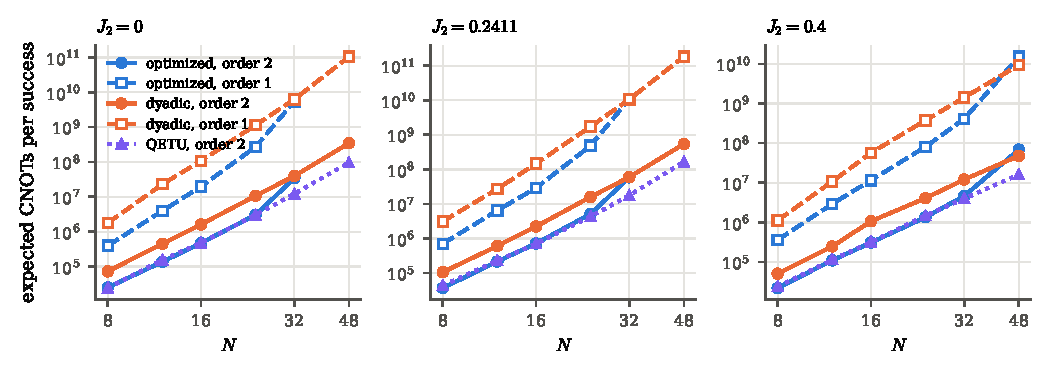
\includegraphics[width=\textwidth]{figs/fig_scaling.pdf}
\caption{Expected CNOTs per successful preparation versus $N$ (trial $\chi=2$, $\epsilon=10^{-2}$),
including the trial circuit and the repetitions (certified success probability). Solid: second order; dashed: first order.
Missing optimized points: no feasible design (see text). Dotted triangles: QETU, second order.
Sources: \texttt{results/scaling.json}, \texttt{results/ext\_qetu\_scaling.json}.}
\label{fig:scaling}
\end{figure*}

\begin{table*}[t]
\caption{Cheapest second-order plan (``sch.'': dyadic or optimized) for $\epsilon=10^{-2}$, trial
$\chi=2$. $\Delta$ is the scaled gap, $T_{\rm phys}=T/W$ in $1/J_1$. Steps for first (1st) and second
(2nd) order with the same schedule; CNOT and $T$ counts for second order per attempt (att.) and per success (succ.), divided by the
certified success probability; ``rot.'': arbitrary rotations per attempt, synthesized to accuracy
$\delta$. Source:
\texttt{results/scaling.json}.}
\label{tab:scaling}
\begin{ruledtabular}
\begin{tabular}{rrrrlrrrrrrrrr}
$N$ & $J_2$ & $\gamma$ & $\Delta$ & sch. & $T_{\rm phys}$ & $p_g$ & steps (1st) & steps (2nd) & CNOT/att. & CNOT/succ. & rot. & $\delta$ & $T$/succ.\\
\midrule
16 & 0 & 0.475 & 0.0206 & opt. & 14.3 & 0.38 & 38{,}020 & 464 & $1.6\times10^{5}$ & $4.2\times10^{5}$ & $7.5\times10^{6}$ \\
16 & 0.2411 & 0.703 & 0.0192 & opt. & 15.0 & 0.58 & 41{,}572 & 521 & $3.6\times10^{5}$ & $6.2\times10^{5}$ & $1.1\times10^{7}$ \\
16 & 0.4 & 0.911 & 0.0211 & opt. & 7.9 & 0.64 & 19{,}266 & 266 & $1.8\times10^{5}$ & $2.8\times10^{5}$ & $5.0\times10^{6}$ \\
24 & 0 & 0.328 & 0.0094 & opt. & 20.5 & 0.27 & 251{,}160 & 1{,}422 & $7.7\times10^{5}$ & $2.9\times10^{6}$ & $5.8\times10^{7}$ \\
24 & 0.2411 & 0.517 & 0.0087 & opt. & 16.3 & 0.29 & 248{,}256 & 1{,}329 & $1.4\times10^{6}$ & $4.8\times10^{6}$ & $1.0\times10^{8}$ \\
24 & 0.4 & 0.839 & 0.0102 & opt. & 13.5 & 0.65 & 87{,}533 & 740 & $7.9\times10^{5}$ & $1.2\times10^{6}$ & $2.3\times10^{7}$ \\
32 & 0 & 0.234 & 0.0054 & opt. & 80.0 & 0.23 & 3{,}103{,}919 & 9{,}847 & $7.2\times10^{6}$ & $3.1\times10^{7}$ & $6.8\times10^{8}$ \\
32 & 0.2411 & 0.373 & 0.0049 & opt. & 85.8 & 0.37 & 4{,}979{,}405 & 13{,}617 & $2.0\times10^{7}$ & $5.3\times10^{7}$ & $1.2\times10^{9}$ \\
32 & 0.4 & 0.768 & 0.0062 & opt. & 16.6 & 0.44 & 221{,}517 & 1{,}305 & $1.9\times10^{6}$ & $4.4\times10^{6}$ & $8.8\times10^{7}$ \\
48 & 0 & 0.125 & 0.0025 & dya. & 146.0 & 0.13 & 20{,}266{,}400 & 34{,}380 & $3.9\times10^{7}$ & $3.1\times10^{8}$ & $7.4\times10^{9}$ \\
48 & 0.2411 & 0.191 & 0.0022 & dya. & 142.5 & 0.19 & 27{,}888{,}279 & 41{,}586 & $9.2\times10^{7}$ & $4.8\times10^{8}$ & $1.2\times10^{10}$ \\
48 & 0.4 & 0.640 & 0.0031 & dya. & 69.3 & 0.64 & 4{,}816{,}485 & 12{,}414 & $2.8\times10^{7}$ & $4.3\times10^{7}$ & $9.9\times10^{8}$ \\

\end{tabular}
\end{ruledtabular}
\end{table*}

\subsection{What if the energy estimates are wrong?}
\label{sec:sens}

The certificate is only as good as its inputs, so we perturb them for $N=12$, $J_2=0.2411$,
$\epsilon=10^{-2}$ (optimized, second order) and simulate the resulting circuit on the true trial state
(Fig.~\ref{fig:sensitivity}).

\begin{figure*}[t]
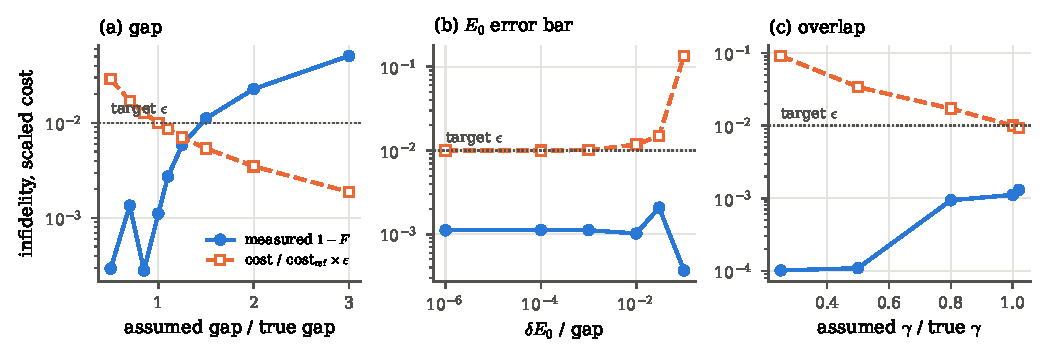
\includegraphics[width=\textwidth]{figs/fig_sensitivity.pdf}
\caption{Sensitivity to the inputs ($N=12$, $J_2=0.2411$, $\epsilon=10^{-2}$). Circles: measured
infidelity of the planned circuit on the true trial state. Squares: expected CNOT cost relative to the
plan with exact inputs, multiplied by $\epsilon$ to share the axis. (a) Assumed gap $f\times$ the
true gap; (b) error bar on $E_0$; (c) assumed overlap $f\times$ the true $\gamma$.
Source: \texttt{results/sensitivity.json}.}
\label{fig:sensitivity}
\end{figure*}

\emph{Gap.} A gap assumed larger than the true one moves the stop-band edge above the first
excitation, which then sits in the filter's transition region. The target was missed in \nGapFail{}
cases, $f\ge\gapFailFactor$, with infidelity up to \gapWorstInf{} at $f=\gapWorstF$; at $f=1.1$ and
1.25 the looseness of the certificate still covered the error. Underestimating the gap is safe and
cheap: even $f=\gapMarginF$ costs only \gapMarginCost$\times$. Since DMRG gives an \emph{upper} bound on $E_1$, an explicit margin $\delta E_1$
is the natural safeguard.

\emph{Ground energy.} An error bar $\delta E_0$ widens the pass band and lowers $F_{\rm pass}$; the
cost stays flat until $\delta E_0$ is a sizeable fraction of the gap (\eZeroHiCost$\times$ at
$\delta E_0=\eZeroHiF$ gap). DMRG energies are far more accurate than this, so $E_0$ is never the
limiting input here.

\emph{Overlap.} Underestimating $\gamma$ is safe (a stricter $\eta$); the planned cost rises
\gammaLowCost$\times$ at $f=0.25$, mostly because the planned success probability $p_g=\gamma F_{\rm
pass}^2$ uses the pessimistic $\gamma$, while the actual success rate does not change. Overestimating
it by 2\% did not break the target in this instance (\nGammaFail{} failures), because the leakage term
is itself loose.

\emph{All instances.} To see whether this one instance is typical we repeated the gap and overlap
perturbations for every $N\le14$, all three couplings and the dyadic, optimized and QETU schedules
(second order, $\epsilon=10^{-2}$; Table~\ref{tab:senswide}). With exact inputs all \sensGapN{} plans
meet the target. An overestimate of the gap by 10\% already breaks it in \sensGapOneTenMiss{} of
\sensGapN{} plans (marginally, worst \sensGapOneTenWorst), by 25\% in \sensGapOneQuarterMiss{} and by
50\% in \sensGapOneHalfMiss. The closed-form dyadic schedule is the most tolerant
(\sensDyaQuarterMiss{} misses at 25\%), because its bound is the loosest; the optimized and Chebyshev
filters, whose leakage terms are nearly tight, have no slack to absorb a wrong gap. Overestimating
$\gamma$ broke the target in \sensGammaMiss{} of \sensGammaN{} plans, all of them through the same
mechanism: the inflated $\gamma$ crossed $1-\epsilon$, so the pipeline dropped the filter altogether
(\sensGammaNoFilter{} of \sensGammaMiss). A margin on both inputs is therefore not optional: $\delta E_1$
should be a sizeable fraction of the gap when $E_1$ is not certified, and the empty filter should be
accepted only on a certified (for example Eckart) lower bound on $\gamma$.

\begin{table}[t]
\caption{Gap and overlap overestimation for every $N\in\{8,10,12,14\}$ and $J_2$ (12 instances),
$\epsilon=10^{-2}$, second order: number of plans that miss the target and the worst measured
infidelity. $f$: assumed over true gap or $\gamma$. Source: \texttt{results/ext\_sensitivity.json}.}
\label{tab:senswide}
\begin{ruledtabular}
\begin{tabular}{lrrrrrrr}
 & & \multicolumn{2}{c}{dyadic} & \multicolumn{2}{c}{optimized} & \multicolumn{2}{c}{QETU}\\
input & $f$ & miss & worst & miss & worst & miss & worst\\
\midrule
gap & 1 & 0/12 & $1.7\times10^{-3}$ & 0/12 & $4.2\times10^{-3}$ & 0/12 & $2.3\times10^{-3}$ \\
gap & 1.1 & 0/12 & $6.5\times10^{-3}$ & 1/12 & $1.1\times10^{-2}$ & 1/12 & $1.0\times10^{-2}$ \\
gap & 1.25 & 0/12 & $6.8\times10^{-3}$ & 5/12 & $2.6\times10^{-2}$ & 5/12 & $3.0\times10^{-2}$ \\
gap & 1.5 & 2/12 & $6.3\times10^{-2}$ & 7/12 & $6.8\times10^{-2}$ & 7/12 & $9.2\times10^{-2}$ \\
gap & 2 & 8/12 & $1.4\times10^{-1}$ & 7/12 & $1.5\times10^{-1}$ & 11/12 & $2.2\times10^{-1}$ \\
gap & 3 & 11/12 & $2.2\times10^{-1}$ & 12/12 & $2.5\times10^{-1}$ & 12/12 & $3.1\times10^{-1}$ \\
$\gamma$ & 1.02 & 1/12 & $2.4\times10^{-2}$ & 1/12 & $2.4\times10^{-2}$ & 1/12 & $2.4\times10^{-2}$ \\
$\gamma$ & 1.05 & 3/12 & $5.5\times10^{-2}$ & 3/12 & $5.5\times10^{-2}$ & 3/12 & $5.5\times10^{-2}$ \\

\end{tabular}
\end{ruledtabular}
\end{table}

\subsection{Choosing the ansatz}
\label{sec:ansatz}

The trial bond dimension trades circuit depth for overlap. Figure~\ref{fig:ansatz} and
Table~\ref{tab:ansatz} show the expected total cost for $\chi=1$ to 8 (the pipeline choosing the
cheaper of the dyadic and optimized schedules). A product state ($\chi=1$) has an exponentially small
overlap and is by far the most expensive start ($10^{7}$--$10^{23}$ CNOTs). Going to $\chi=2$ and
$\chi=4$ lowers the cost by orders of magnitude: at $N=48$, $J_2=0.2411$ the $\chi=4$ plan needs
\cnotFortyEightChiFour{} CNOTs and \tFortyEightChiFour{} $T$ gates per success. At $\chi=8$ the trial
state alone satisfies $1-\gamma\le10^{-2}$ in \nNoFilterChiEight{} of \nChiEight{} cases
($\gamma=\gammaFortyEightChiEight$ at $N=48$, $J_2=0.2411$), and the pipeline returns the empty filter:
\cnotFortyEightChiEight{} CNOTs. For this gapless-to-weakly-gapped one-dimensional chain at
$\epsilon=10^{-2}$, directly compiling a better MPS is therefore much cheaper than filtering a worse
one. The filter becomes the better
tool when the target is tighter than what a compilable MPS reaches, when a certificate on the output
is required, or when the classical method cannot provide a compact high-overlap trial circuit, as for
two-dimensional lattices.

\begin{figure*}[t]
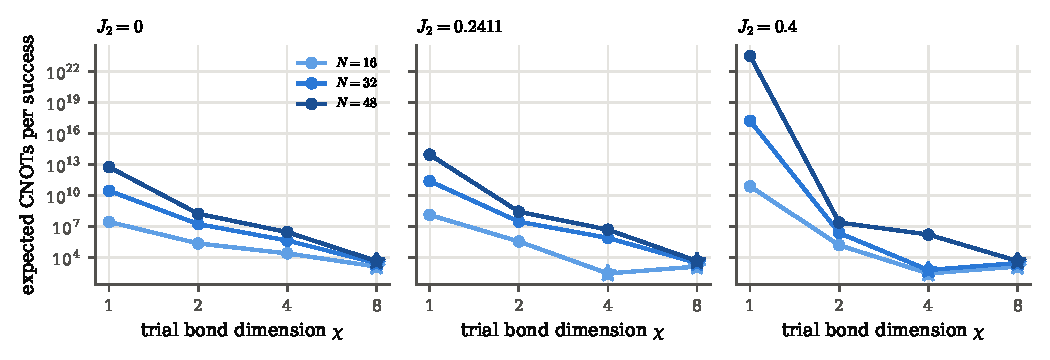
\includegraphics[width=\textwidth]{figs/fig_ansatz.pdf}
\caption{Expected CNOTs per success versus trial bond dimension ($\epsilon=10^{-2}$, second order,
cheaper of dyadic and optimized). Stars: the trial state alone satisfies $1-\gamma\le\epsilon$ and no
filter is used. Source: \texttt{results/ansatz.json}.}
\label{fig:ansatz}
\end{figure*}

\begin{table*}[t]
\caption{Overlap $\gamma$ and expected CNOTs per success for trial bond dimension $\chi=1,2,4,8$
($\epsilon=10^{-2}$, second order, cheaper schedule; no filter when $1-\gamma\le\epsilon$).}
\label{tab:ansatz}
\begin{ruledtabular}
\begin{tabular}{rrrrrrrrrr}
$N$ & $J_2$ & $\gamma_1$ & CNOT & $\gamma_2$ & CNOT & $\gamma_4$ & CNOT & $\gamma_8$ & CNOT\\
\midrule
16 & 0 & 0.028 & $2.8\times10^{7}$ & 0.475 & $2.3\times10^{5}$ & 0.984 & $2.5\times10^{4}$ & 1.000 & $1.3\times10^{3}$ \\
16 & 0.2411 & 0.019 & $1.3\times10^{8}$ & 0.703 & $3.5\times10^{5}$ & 0.998 & $2.8\times10^{2}$ & 1.000 & $1.3\times10^{3}$ \\
16 & 0.4 & 0.000 & $7.6\times10^{10}$ & 0.911 & $1.5\times10^{5}$ & 0.999 & $2.8\times10^{2}$ & 1.000 & $1.3\times10^{3}$ \\
32 & 0 & 0.001 & $2.8\times10^{10}$ & 0.234 & $1.7\times10^{7}$ & 0.913 & $4.3\times10^{5}$ & 0.998 & $2.9\times10^{3}$ \\
32 & 0.2411 & 0.001 & $2.5\times10^{11}$ & 0.373 & $2.9\times10^{7}$ & 0.972 & $7.7\times10^{5}$ & 0.999 & $2.9\times10^{3}$ \\
32 & 0.4 & 0.000 & $1.7\times10^{17}$ & 0.768 & $2.3\times10^{6}$ & 0.990 & $6.0\times10^{2}$ & 1.000 & $2.9\times10^{3}$ \\
48 & 0 & 0.000 & $5.5\times10^{12}$ & 0.125 & $1.7\times10^{8}$ & 0.817 & $2.8\times10^{6}$ & 0.990 & $4.5\times10^{3}$ \\
48 & 0.2411 & 0.000 & $9.0\times10^{13}$ & 0.191 & $2.7\times10^{8}$ & 0.920 & $4.8\times10^{6}$ & 0.995 & $4.5\times10^{3}$ \\
48 & 0.4 & 0.000 & $3.2\times10^{23}$ & 0.640 & $2.4\times10^{7}$ & 0.976 & $1.6\times10^{6}$ & 0.998 & $4.5\times10^{3}$ \\

\end{tabular}
\end{ruledtabular}
\end{table*}

\subsection{Measured crossover}
\label{sec:crossover1d}

The comparison above is certified on both sides only for the MPS. To compare like with like we measure the
filtered route too: for chains of $N=12$--16 at $J_2=0$, 0.2411 and 0.4, the exact spectrum of each
Hamiltonian is computed per $S^z$ block, every MPS trial with $\chi=2,\dots,64$ is decomposed on it, and for
each target $\epsilon\in[10^{-5},10^{-2}]$ the cheapest route is found: the smallest MPS that meets
$1-\gamma\le\epsilon$ alone, against the cheapest smaller MPS followed by a measured dyadic or optimized SBC
filter (shortest exact ladder or design, then the coarsest passing Strang step), with cost (trial $+$
filter)$/p$.

Figure~\ref{fig:actual1d} shows the result on nine chains. Compiling the MPS directly is the cheaper route
in most cases: the filtered route wins in \actOneWins{} of the \actOneTot{} (chain, $\epsilon$) targets, by
1.1--\actOneRatioMax$\times$. The wins share a single mechanism. Because MPS compilation cost jumps with
$\chi$ (here by a factor of about four from $\chi=4$ to 8 and from 8 to 16), a target lying just below what a
given $\chi$ reaches forces the MPS-alone route up to the next bond dimension, while the trial at the lower
$\chi$ misses the target only slightly. All \actOneNearWins{} wins filter such a trial, with
$(1-\gamma)/\epsilon\le\actOneFarMax$ (13 of them below 3), using a dyadic ladder of one to four pulses ($K\le3$,
$r\le2$, 1--21 Strang steps) that succeeds with $p\ge0.988$. Of the \actOneNear{} filtered routes with
$(1-\gamma)/\epsilon\le\actOneFarMax$, \actOneNearWins{} beat the MPS alone; all \actOneFar{} with a larger
ratio lose, by a median factor of \actOneFarMed. In this regime the filter acts as a last-mile polisher: it
removes the residual infidelity of a nearly sufficient trial, but recovering a larger factor is cheaper by
doubling $\chi$. The location of the wins in $\epsilon$ therefore depends on the system through where each
$\chi$ lands, not on $N$ or $J_2$ in any simple way, and an MPS with intermediate bond dimension (not tried
here) would compete with some of them. The optimized design never wins. A single dyadic pulse lasts only
$\pi/(1+\Delta)$ and keeps $f(E_0)=1$; it does not resolve the gap, but it removes 17--68\% of the residual
weight, which suffices for a trial this close to the target. The optimized design certifies suppression on the
whole band above $\Delta$ and so needs $T\gtrsim\pi/\Delta$: rerunning the competitive cases
($(1-\gamma)/\epsilon\le20$; 32 of 40 completed) with one- to three-pulse designs and the design target loosened up
to $10\epsilon$ lowered its cost by up to $3\times$ but left $T=35$--66 against 3--21 for the winning dyadic
ladders, and it beat the dyadic route in 3 of the 23 cases with $(1-\gamma)/\epsilon\le\actOneFarMax$ and the MPS
alone in none (\texttt{results/emp\_actual1d\_opt.jsonl}). QETU beats the MPS alone in 11 of the targets but is
never the cheapest route. This matches the observation for rodeo filters that a ratio-2 time series is optimal
when the total time is short and longer series favor other designs~\cite{Patkowski2026}. Because the bond
dimension a chain needs for fixed $\epsilon$ grows only slowly with $N$, we expect this picture to hold for longer
chains; on cylinders it reverses (Sec.~\ref{sec:twod}).

\begin{figure*}[t]
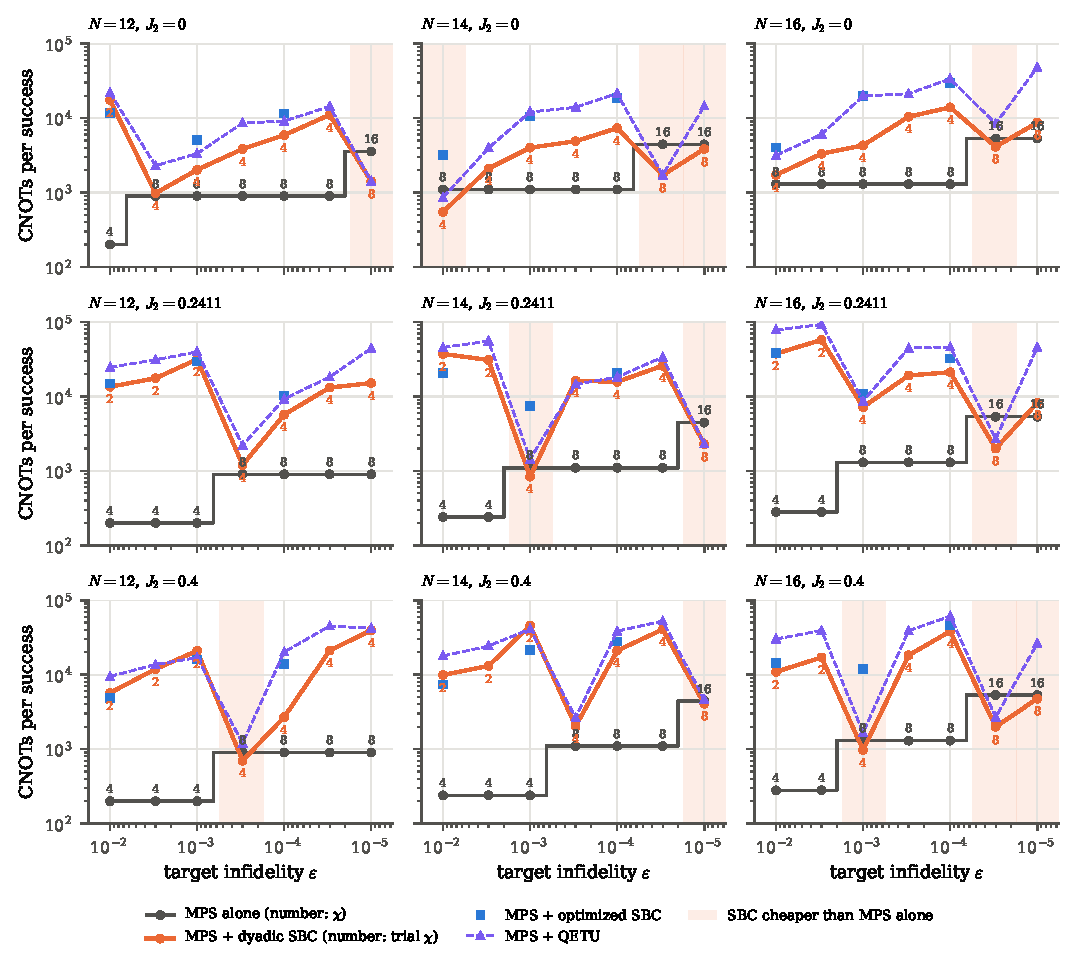
\includegraphics[width=\textwidth]{figs/fig_actual1d.pdf}
\caption{Measured cheapest route to infidelity $\epsilon$ on chains of $N=12$, 14, 16 (columns) at $J_2=0$,
0.2411, 0.4 (rows), all by exact simulation. Grey: cheapest MPS that meets $1-\gamma\le\epsilon$ alone (number:
$\chi$). Orange: cheapest smaller MPS followed by the dyadic SBC filter (number: trial $\chi$); blue squares:
optimized SBC (designed at $\epsilon=10^{-2},10^{-3},10^{-4}$ only); purple: QETU. Shaded: the SBC route is
cheaper. Cost is (trial $+$ filter CNOTs)$/p$. Sources: \texttt{results/emp\_actual1d.jsonl} and, for
$N=16$, $J_2=0.2411$, \texttt{results/emp\_actual.json}.}
\label{fig:actual1d}
\end{figure*}

%=====================================================================================================%=====================================================================================================
\section{Two dimensions: where the filter pays}
\label{sec:twod}

The pipeline is generic in $H$, so we ran the measured crossover of Sec.~\ref{sec:crossover1d} on the
$J_1$--$J_2$ model on $4\times3$ and $4\times4$ cylinders (periodic around the four-site circumference, open
along $L_x$) at $J_2=0$ and 0.3, with snake-path MPS trials up to $\chi=64$ and exact spectra
(Fig.~\ref{fig:actual}). Cylinders are much harder for a snake MPS than chains. At $4\times4$, $J_2=0$, the
$\chi=16$ trial still misses $\epsilon=10^{-2}$ ($1-\gamma=1.1\times10^{-2}$), $\chi=32$ stalls at
$7\times10^{-4}$, and no $\chi\le64$ trial reaches $10^{-5}$ ($1-\gamma\approx2\times10^{-5}$ at $\chi=64$), while
the compile cost grows about fourfold per doubling of $\chi$ (5\,328, 20\,548 and 76\,600 CNOTs for
$\chi=16$, 32, 64). On $4\times3$, $\chi=64$ is exact, but only at 45\,960 CNOTs.

The result is the opposite of the chain. The filtered route is cheaper at 27 of the 28 cylinder targets
from $\epsilon=10^{-2}$ to $10^{-5}$, by 1.1--\actRatioMax$\times$ where both routes exist, and it is
the only route at $10^{-5}$ on $4\times4$. The exception is $\epsilon=10^{-2}$ on $4\times4$, $J_2=0.3$, where the
$\chi=16$ MPS alone already reaches $8.3\times10^{-3}$. Every win uses the dyadic ladder, on a $\chi=16$ trial
in 24 of the 27 (otherwise $\chi=4$, 8 or 32), with $p\ge0.77$ and 1--46 Strang steps. Unlike the chain, the filter here recovers large factors:
the trials miss the target by $(1-\gamma)/\epsilon$ up to $10^3$, and the advantage grows toward tight targets
(up to $8.8\times$ at $4\times4$, $J_2=0$, $\epsilon=3\times10^{-4}$, where $\chi=16$ plus 10 Strang steps replaces
$\chi=64$). Two properties of the filter carry this: its depth grows only with $\ln(1/\epsilon)$ at a
fixed gap, while the MPS needed to reach $\epsilon$ alone grows by a factor of four per bond-dimension step,
and its cost in the overlap is the logarithm of Sec.~\ref{sec:gapov}. On the 16-site chain in the same
comparison the filter wins only at $\epsilon=3\times10^{-5}$ and $10^{-5}$. The result depends on the MPS circuit cost, which we take from the generic
quantum-Shannon bound. Table~\ref{tab:robust} re-costs every MPS circuit, in both routes, with a factor $f\le1$
and with the lower bound for isometries from $b$ to $b+1$ qubits~\cite{Iten2016}, $\lceil(3\cdot4^b-b-2)/4\rceil$
CNOTs per site (about 0.4 of the bound used), which no compiler of these site unitaries can beat. At that lower
bound the filter still wins \robLbTwo{} of the 28 cylinder targets, and it keeps a majority until MPS circuits are
about eight times cheaper than the bound we use; on chains its \actOneWins{} wins fall to \robLbOne. Over these
targets the cylinder result is therefore robust to the MPS compiler; the chain result is not. These are small
cylinders, at sizes where exact simulation is possible, and we leave a systematic two-dimensional study to future work; with certified plans
in place of measured ones, the same comparison extended to $4\times12$ finds the filter to be the only route at
$\epsilon=10^{-4}$ on the larger cylinders. For the two-dimensional $J_1$--$J_2$ model, resource estimates
for phase estimation have assumed the state preparation to be negligible~\cite{Yoshioka2024}; these results
suggest that a compiled low-$\chi$ MPS plus a short filter is a practical way to meet that assumption.

\begin{figure*}[t]
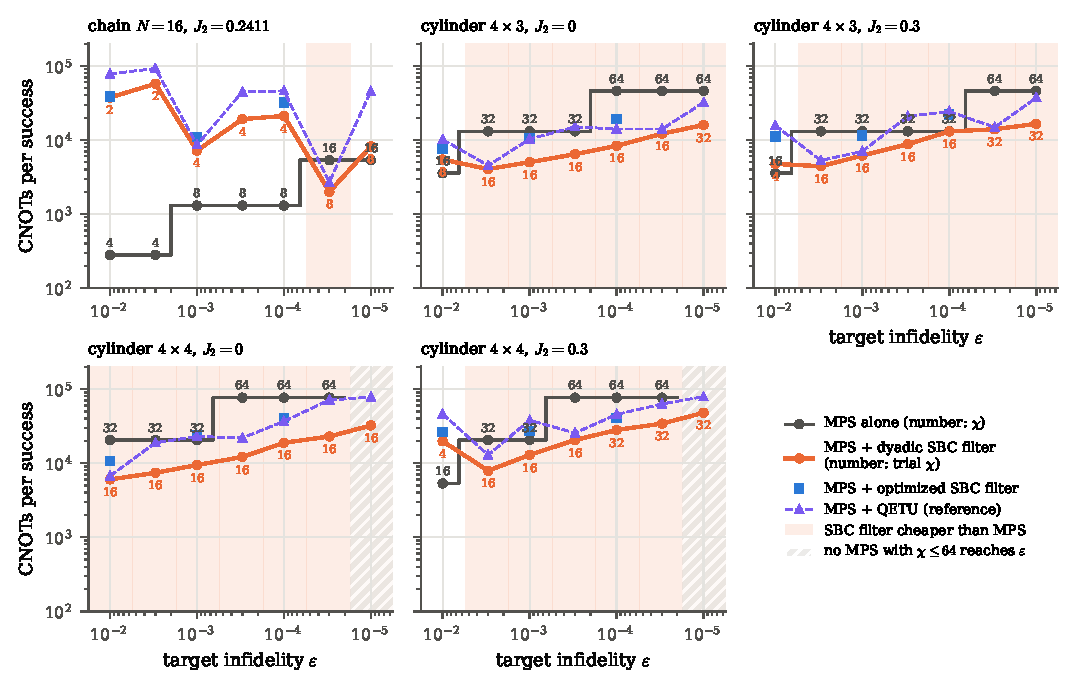
\includegraphics[width=\textwidth]{figs/fig_actual.pdf}
\caption{Measured cheapest route to infidelity $\epsilon$ on the 16-site chain and on small cylinders. Grey:
the cheapest MPS that meets the target alone (number: $\chi$). Orange: the cheapest smaller MPS followed
by the dyadic SBC filter (number: trial $\chi$); blue squares: optimized SBC; purple: QETU. Shaded:
the filtered route is cheaper; hatched: no MPS with $\chi\le64$ reaches $\epsilon$. Every cost is (trial $+$
filter CNOTs)$/p$ from exact simulation. Source: \texttt{results/emp\_actual.json}.}
\label{fig:actual}
\end{figure*}

\begin{table}[t]
\caption{Robustness of the measured crossovers to the cost of the MPS circuits: targets (of 28 cylinder and 63
chain targets) at which MPS + SBC filter beats the MPS alone when every MPS circuit is re-costed by a factor $f$,
with the quantum-Shannon bound used throughout and with the isometry lower bound~\cite{Iten2016}.}
\label{tab:robust}
\begin{ruledtabular}
\begin{tabular}{lrrrrr}
MPS cost model & $f=1$ & $1/2$ & $1/4$ & $1/8$ & $1/16$\\
\midrule
QSD bound (used), cylinders (of 28) & 27 & 25 & 23 & 19 & 13 \\
QSD bound (used), chains (of 63) & 18 & 13 & 6 & 4 & 0 \\
isometry lower bound, cylinders (of 28) & 24 & 22 & 18 & 12 & 9 \\
isometry lower bound, chains (of 63) & 11 & 6 & 4 & 0 & 0 \\

\end{tabular}
\end{ruledtabular}
\end{table}

%=====================================================================================================
\section{Comparison with a Chebyshev filter (QETU)}
\label{sec:qetu}

To compare with a polynomial filter under the same accounting, the pipeline also
designs the quantum eigenvalue transformation of unitaries (QETU) of Dong, Lin and Tong~\cite{Dong2022}.
It uses the same primitive, $d$ queries of $e^{-i\tau H_s\otimes Z_a}$, the controlled-reversal form
also used by the rodeo algorithm~\cite{BeeLindgren2025}, but interleaves them with ancilla rotations
and post-selects only once. On every eigenvector the ancilla then undergoes quantum signal processing in
$x=\cos(\tau E)$, so the ancilla-0 block is $p(\cos\tau H_s)$ for any real even polynomial $p$ of degree
$d$ with $|p|\le1$ on $[-1,1]$~\cite{Dong2022}. With $\tau=\pi/2$ the scaled spectrum maps to $x\in[0,1]$
and the stop band to $[0,x_s]$, $x_s=\cos(\pi\Delta/2)$. We take the Chebyshev filter
\begin{equation}
p(x)=\frac{T_d(x/x_s)}{T_d(1/x_s)},\qquad \eta=\frac1{T_d(\cos(\tau w_0)/x_s)},
\end{equation}
which is extremal: no polynomial of degree $d$ bounded by 1 is smaller on the stop band relative to its
value at the pass band. It is certified in closed form ($p$ is monotone on $[x_s,1]$ and equioscillates
on $[-x_s,x_s]$), has $p(0)=1$ so $p_g=\gamma F_{\rm pass}^2\approx\gamma$, and needs
$T=d\tau\approx\Delta^{-1}\ln(2/\eta)$, two to three times less than the dyadic ladder. The Trotter bound,
step allocation and Theorem~\ref{thm:cert} carry over unchanged, with one pulse per query and two ancilla
rotations per query (the phase and the identity term). The QSP phases are computed classically; our
cost model does not include that step. For second-order formulas $S_2(-\tau)=S_2(\tau)^\dagger$, so the
Trotterized circuit implements exactly $p(\tilde X)$ with $\tilde X=\frac12(S_2(\tau)+S_2(-\tau))$, which is
how we simulate it; the test suite checks this against an explicit ancilla circuit with QSP phases.

\emph{Certified.} The Chebyshev QETU filter, planned with the same Trotter, synthesis and
cost model, is feasible in all \qetuN{} second-order cases (\qetuFail{} failures) and is a median
\qetuDyaMed$\times$ (range \qetuDyaMin--\qetuDyaMax) cheaper than the dyadic schedule. Against the
optimized SBC design, where that design exists, the ratio is a median \qetuOptMed{} (range
\qetuOptMin--\qetuOptMax, \qetuOptN{} cases): the two cost the same to within the spread, because both
reach $T\approx\Delta^{-1}\ln(1/\eta)$ up to a constant and the Trotter cost depends only on $T$. At
$N=48$, $J_2=0.2411$ QETU needs \qetuFortyEight{} CNOTs per success against \cnotFortyEight{} for the
dyadic plan (Fig.~\ref{fig:scaling}). Simulated as in Sec.~\ref{sec:validation}, the certificate held in
\qetuNSimOK{} of \qetuNSim{} QETU plans ($N\le14$, both targets), with a median looseness of
\qetuBoundMed$\times$; its leakage term is tight (median \qetuLeakMed$\times$) because the Chebyshev
filter equioscillates across the stop band. In the controlled study of Sec.~\ref{sec:gapov}, the certified QETU
plan is a median \cQetuOverDyMed{} times the certified dyadic one and cheaper in all \cQetuWinsDy{} cases, and it is
the cheapest certified filter in \cbestQeTwo, \cbestQeThree{} and \cbestQeFour{} of 74 cases at
$\epsilon=10^{-2}$, $10^{-3}$, $10^{-4}$ (the optimized SBC design takes the rest). Certified, the SBC filter therefore offers no cost advantage over a
polynomial filter; what it offers is the absence of a phase-finding step and a measurement after every
pulse, which an early-abort protocol (not modeled here) could exploit.

\emph{Measured.} The gap/overlap study simulates both filters on every case
(Figs.~\ref{fig:filterA}--\ref{fig:mech}, bottom rows and purple points). Measured, the dyadic SBC filter is
the cheaper one at loose targets: QETU is cheaper in \goQetuWinsTwo{} of \goCasesTwo{} cases at
$\epsilon=10^{-2}$, \goQetuWinsThree{} of \goCasesThree{} at $10^{-3}$, but \goQetuWinsFour{} of
\goCasesFour{} at $10^{-4}$; over all cases QETU costs a median \goQetuOverDyMed$\times$ the dyadic filter.
The reason is the Trotter step, not the filter. QETU needs less evolution time (a median \fQDtime$\times$
the dyadic time), but it must take one fine Strang step per short query, $\delta t=\tau/W\propto1/N$, so its
step count is a median \fQDsteps$\times$ the dyadic one and its CNOTs grow as $N^{\fitMQCN}$ against
$N^{\fitMDCN}$. The long dyadic pulses tolerate steps of order $1/J_1$, but these shrink as roughly
$\epsilon^{0.3}$, and by $\epsilon=10^{-4}$ the shorter QETU filter wins. QETU's measured cost is also the more
regular of the two (Table~\ref{tab:gofit}): its fit holds to \goMQrms$\times$, because its degree grows by
two at a time where the dyadic ladder grows in whole pulses.

\subsection{What the Chebyshev filter needs}
\label{sec:empirical}

To see how the gap and the overlap act on the Chebyshev filter itself, we replace the certificate
by simulation for $N=8$--16 (\empN{} cases). Each trial state is decomposed on the exact eigenbasis
(dense diagonalization per $S^z$ block), so the smallest QETU degree $d_{\min}$ that reaches $\epsilon$ for
that state is found exactly; at that degree we then find the smallest number of Strang steps per
query with the Trotterized circuit simulated on the full state vector, allowing a slightly higher
degree when it makes one step per query enough. Three families separate the inputs. In the first,
$J_2=0.2411$ for every $N$ and the gap closes with $N$. In the second, $J_2$ is chosen at each $N$ (by
bisection on ED) so that the gap is $E_1-E_0=0.40$ exactly ($J_2=\empMatchJ$ for $N=8$--16). In the
third, $J_2$ is tuned at $N=10$, 12 and 14 to gaps from 0.30 to 0.55. For the trial states we use the
optimal MPS at $\chi=1$, 2, 4 and synthetic states $\sqrt{\gamma}|E_0\rangle+\sqrt{1-\gamma}|\xi\rangle$ with
$\gamma$ from 0.03 to 0.9, $\xi$ being the normalized excited part of the $\chi=2$ MPS, so that the overlap
changes while the shape of the excited weight does not. $\epsilon\in\{10^{-2},10^{-3},10^{-4}\}$.

\emph{The degree is set by the gap and the target alone.} The measured degrees collapse onto
\begin{equation}
d_{\min}\,\Delta\;\simeq\;\frac{2}{\pi}\cosh^{-1}\frac1\eta,\qquad \eta^2=\frac{\gamma\epsilon}{1-\gamma},
\label{eq:dmin}
\end{equation}
for every family, trial and target (Fig.~\ref{fig:empirical}b). This is the certified degree with the
true gap: the certificate asks for a median \empDegRatio{} times $d_{\min}$. Where the excited weight
of the trial sits does not help. The Chebyshev filter is equiripple, so every state above the gap is
suppressed by the same factor $1/T_d(1/x_s)$, and a trial whose excited weight lies far above the gap
needs the same degree as one whose weight sits at the gap. Over the gap scan $d_{\min}\propto\Delta^{-\empGapDeg}$.

\emph{The certificate's Trotter count is pessimistic, not its filter.} One Strang step per query was
enough in all \empKone{} cases, against a certified median of \empCertK{} steps per query. Commutator
bounds are worst-case over all states, but the filter only has to act well on a state supported near
the bottom of the spectrum. As a result the certified cost is a median \empCertRatio{} times what the
filter needs (range \empCertRatioMin--$\empCertRatioMax$), and the real cost follows the degree:
\begin{equation}
\text{cost}_{\rm real}\;\approx\;\frac{c_{\rm step}(N)}{\gamma}\,d_{\min}
\;\propto\;\frac{c_{\rm step}(N)\,W}{g\,\gamma}\,\ln\frac{1-\gamma}{\gamma\epsilon},
\label{eq:costreal}
\end{equation}
with $c_{\rm step}$ the CNOTs of one step ($\propto N$) and $g=E_1-E_0$. Fitting the simulations gives
overlap $\gamma^{-\empGamLog}$ once the logarithm is divided out ($\gamma^{-\empGamRaw}$ as a plain power,
against $\gamma^{-\empGamCert}$ for the certified plan) and gap $\Delta^{-\empGapExp}$ (certified
$\Delta^{-\empGapCert}$). With the gap held at 0.40 the cost grows as $N^{\empNMatch}$; at fixed $J_2$,
where $g$ also closes, as $N^{\empNFixed}$ (Fig.~\ref{fig:empirical}c). The difference is the
$1/g$ of Eq.~\eqref{eq:costreal}.

\emph{Gap and overlap are not independent inputs.} Tuning $J_2$ to hold the gap moves the chain toward
the dimerized point $J_2=1/2$, where a $\chi=2$ MPS is close to exact: at the gap-matched couplings the
$\chi=2$ overlap is 0.97--1.00 at every $N$, against 0.70--0.90 at $J_2=0.2411$. Up to $J_2\approx1/2$ a larger gap and a better
trial come together, so for real trials the two effects compound; beyond it the gap keeps
growing while the $\chi=2$ overlap falls again (to 0.78 at $J_2=0.68$, $N=14$). Holding one of them fixed
through $J_2$ therefore always moves the other, which is why the scans here use synthetic trials and
Sec.~\ref{sec:gapov} a sublattice rotation of a real trial circuit.

\begin{figure*}[t]
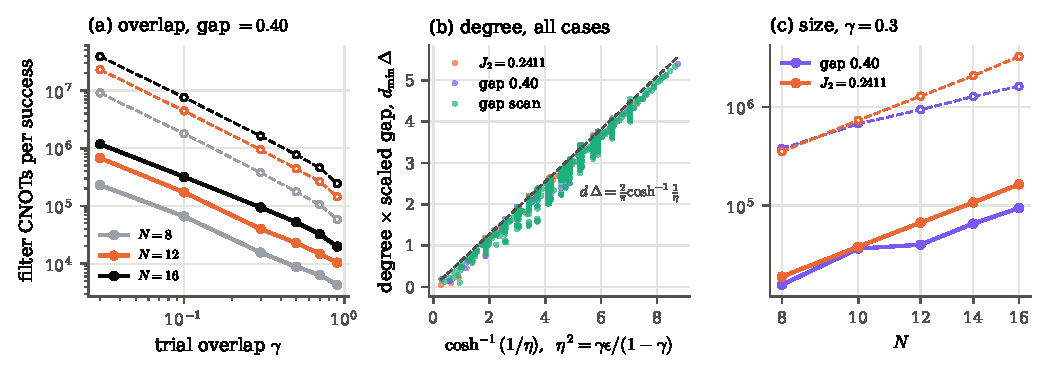
\includegraphics[width=\textwidth]{figs/fig_empirical.pdf}
\caption{What the filter actually needs, from exact spectra and state-vector simulation ($N=8$--16,
QETU, second order). (a) CNOTs per success versus overlap at a gap held at 0.40, $\epsilon=10^{-3}$:
simulated (filled) and certified (open, dashed). (b) Smallest degree times scaled gap for all \empN{}
cases against $\cosh^{-1}(1/\eta)$; dashed: Eq.~\eqref{eq:dmin}. (c) Cost versus $N$ at $\gamma=0.3$,
$\epsilon=10^{-3}$, with the gap held at 0.40 or $J_2$ held at 0.2411. Source:
\texttt{results/emp\_trotter.json}, \texttt{sbpipe\_study/run\_empirical.py}.}
\label{fig:empirical}
\end{figure*}


%=====================================================================================================
\section{Measured versus certified}
\label{sec:meascert}

Every comparison above has two versions, and they do not always agree (Table~\ref{tab:meascert}). The
measured cost is not implementable as it stands: it picks the shortest filter and the coarsest Trotter step
that reach $\epsilon$ for the given trial, which needs the exact ground state. It is the cost an ideal
a-posteriori procedure could approach, and it shows what the circuit actually has to do. The certified cost is
what the pipeline plans from Theorem~\ref{thm:cert} without that knowledge, and can be run as is. The two
differ mainly through the Trotter step (Sec.~\ref{sec:gapov}): the certified step is 60--75 times finer, and its
overhead grows with the filter length.

This difference decides which filter is cheapest. Measured, the long SBC pulses tolerate steps of order
$1/J_1$ and win at loose targets; certified, every filter pays the same worst-case step per unit time, the
shorter Chebyshev filter wins more often, and the optimized SBC design is the only one that competes. It also
decides the end-to-end comparison. Certified, the filtered route is 1--2 orders of magnitude more expensive
than measured. Against compiling a better MPS it loses at all 63 chain targets (median \certOneOverMed$\times$
the MPS cost, never below \certOneOverMin$\times$) and at every cylinder target where some $\chi\le64$ reaches
$\epsilon$ (median \certTwoOverMed$\times$), with one exception: QETU on $4\times3$, $J_2=0$, at $\epsilon=10^{-4}$,
which is $1.2\times$ cheaper and where the SBC filter ties. It remains the only route where no MPS reaches the target. The measured cylinder advantage is
therefore a statement about what the circuit needs, which an implementation can claim only with a tighter
error bound, for example one restricted to the low-energy subspace~\cite{Sahinoglu2021,Mizuta2025}, or with an
a-posteriori check of the Trotter step (shrinking it until a measured energy or fidelity proxy stops changing).
Two smaller oracle elements are the exact gap and overlap used to design the measured filters; the sensitivity
study of Sec.~\ref{sec:sens} shows that an overestimated gap is the dangerous error, so a margin on $E_1$ is
needed in practice.

\begin{table}[t]
\caption{Each comparison measured (shortest filter and coarsest Trotter step that reach $\epsilon$ in exact
simulation; uses the ground state) and certified (planned from Theorem~\ref{thm:cert}; implementable).
Controlled study: 74 cases per target. Crossovers: targets $10^{-2}$--$10^{-5}$; certified SBC uses the
pipeline's automatic choice of dyadic or optimized, QETU in parentheses. Sources: \texttt{results/gapov*.jsonl},
\texttt{results/emp\_actual*.json*}, \texttt{results/cert\_crossover.jsonl}.}
\label{tab:meascert}
\begin{ruledtabular}
\begin{tabular}{p{4.2cm}ll}
comparison & measured & certified\\
\midrule
Cheapest filter, $\epsilon=1\times10^{-2}$ (dy/opt/QETU) & 23/51/0 & 0/38/36 \\
Cheapest filter, $\epsilon=1\times10^{-3}$ (dy/opt/QETU) & 16/57/1 & 0/25/49 \\
Cheapest filter, $\epsilon=1\times10^{-4}$ (dy/opt/QETU) & 5/32/37 & 0/0/74 \\
MPS + filter beats MPS alone, 9 chains & 18 of 63 & 0 of 63 (QETU 0) \\
MPS + filter beats MPS alone, 4 cylinders & 27 of 28 & 2 of 28 (QETU 3) \\

\end{tabular}
\end{ruledtabular}
\end{table}

%=====================================================================================================
\section{Discussion}

\emph{What makes the filter advantageous.} The controlled study separates three regimes. (i) The gap
determines the coherent circuit: evolution time $\propto L/\Delta$, independent of $N$ at fixed gap, and
CNOTs and $R_z$ per shot that scale as a power of $1/\Delta$. A system with a large gap in absolute units is
the natural target, and the filter's depth is what hardware with a coherence or logical-error budget has to
accommodate. (ii) The trial overlap enters the circuit only through a logarithm and the expected cost through
$1/\gamma$: the filter is tolerant of a poor trial, paying in repetitions rather than in depth. This is
where it has an edge over compiling a better trial, whose cost grows with the bond dimension needed to
reach $\epsilon$ directly. (iii) The target enters through $L$ and, for SBC, through the Trotter step,
$\delta t\propto\epsilon^{0.3}$; tight targets are where a compiled MPS runs out first. For the chain, the MPS
infidelity falls quickly with $\chi$, so the filter pays off only as a last-mile polisher, on a trial within a
factor of about \actOneFarMax{} of the target (Sec.~\ref{sec:crossover1d}); for cylinders, where a
snake MPS struggles, it pays off at 27 of the 28 targets we measured (Sec.~\ref{sec:twod}).

\emph{Dyadic, optimized or Chebyshev.} Both SBC schedules beat the Chebyshev filter at
$\epsilon\ge10^{-3}$, measured (certified, the Chebyshev filter is usually the cheaper one,
Sec.~\ref{sec:meascert}), because their long smooth pulses tolerate Trotter steps of order $1/J_1$;
the Chebyshev filter is shorter and catches up at $\epsilon=10^{-4}$. The optimized SBC design is the cheapest of the three at
$\epsilon\le10^{-3}$ in most cases, measured (median \odMMed$\times$ dyadic) and even more so certified
(\odCMed$\times$), but it needs a numerical design that occasionally fails and must be repeated; the dyadic
ladder is the robust default and the natural fallback, which is how the pipeline's ``auto'' mode uses
them.

\emph{Amplitude amplification.} All costs here are repeat-until-success, $C/p$ per success. Amplitude
amplification~\cite{Brassard2002} would instead run the filter coherently about $\pi/(4\sqrt p)$ times, each round
costing the trial and filter circuits and their inverses, for an expected cost near $(\pi/2)C/\sqrt p$: a
saving of about $(\pi/2)\sqrt p$, i.e.\ worthwhile only for $p\lesssim0.4$. At the lowest overlap of the controlled
study ($p\approx\gamma=0.03$) it would cut the cost per success by about $3.7\times$, at the price of a coherent
circuit about six times deeper, which works against the depth budget the gap already sets. Two further costs apply
to the cosine filter. The SBC circuit measures the ancilla after every pulse; a coherent version needs one ancilla
per pulse (or the pulses combined into a single post-selection, as in QETU), and with $p$ known only as an estimate
a fixed-point variant~\cite{Yoder2014} is needed, which costs a further logarithmic factor. Where the filter
wins in the crossovers, the trial is good and $p\ge0.77$, so amplification would not help; it matters in the
low-overlap regime, where it changes the $1/\gamma$ of the cost laws into $1/\sqrt\gamma$. An early-abort protocol
that stops at the first failed pulse is the cheaper complement for SBC and is likewise not modeled.

\emph{What is guaranteed.} Theorem~\ref{thm:cert} holds whenever its inputs are right. Of these, the
spectral upper bound (Weyl) and the filter certificate are rigorous, and the Trotter constants are exact up to
the Lanczos tolerance of their largest local norms. The interval for $E_0$, the lower bound on $E_1$ and the
overlap $\gamma$ come from DMRG and are well-converged estimates, not bounds; for $N\le14$ ED confirms them,
beyond that the certificate is conditional on all three. The gap is the critical input: an overestimate of
10--25\% already broke the target for the optimized and Chebyshev filters (Table~\ref{tab:senswide}).
Rigorous lower bounds on $E_1$ (e.g.\ Temple-type bounds) would remove the gap condition, and with them the
Eckart inequality $1-\gamma\le(\langle H\rangle_\psi-E_0)/(E_1-E_0)$ would remove the overlap condition.

\emph{Where the certified cost goes.} The certified filter length is within a factor of about two of what
simulation needs; the certified Trotter step is 60--75 times finer than needed, and the certified step
count grows as $L^{2}$ rather than $L$. Tighter Trotter bounds, for example restricted to the low-energy
subspace~\cite{Sahinoglu2021,Mizuta2025}, or a posteriori error estimates, would recover most of the \goCertRatioMed-fold
median gap between certified and measured cost; a better filter design would not.

\emph{Limitations.} Noiseless simulation; repeat-until-success rather than early abort; all-to-all
connectivity (a nearest-neighbor layout would add SWAPs, mostly for the ancilla, which couples to every bond); trial circuits costed by a generic
decomposition bound rather than compiled; exact simulation and the controlled study only up to $N=14$--16, so
the fitted exponents are descriptive; the gap range that can be held fixed across $N$ is narrow
(0.30--0.55); $E_1$ is taken as the lowest $S^z=1$ state, which is the first excitation in every ED case here
but an assumption for larger $N$.

%=====================================================================================================
\section*{Code and data availability}
The \texttt{sbpipe} package, the study scripts, all raw results (\texttt{sbpipe\_study/results/*.json}) and
the sources of this paper are available at \url{https://github.com/aaronseymour7/FilterPipeline}.

\appendix

\section{Proof of Theorem~\ref{thm:cert}}
\label{app:proof}

Write the trial state as $\ket\psi=\sqrt{\gamma'}\ket g+\sqrt{1-\gamma'}\ket\chi$ with $\ket g$ in the
ground space (energy $e_0\in[0,w_0]$ in scaled units), $\ket\chi$ orthogonal to it and $\gamma'\ge\gamma$.

\begin{lemma}[leakage]\label{lem:leak}
For the exact filter, $v=F(H_s)\ket\psi$ has weight outside the ground space at most $\ell$, and
$\norm v^2\ge p_g$.
\end{lemma}
\begin{proof}
$F(H_s)$ is a function of $H_s$, so $v=\sqrt{\gamma'}F(e_0)\ket g+\sqrt{1-\gamma'}F(H_s)\ket\chi$ with
the two parts orthogonal. Every component of $\ket\chi$ has energy in $[\Delta,1]$, so
$\norm{F(H_s)\chi}\le\sup_{[\Delta,1]}|F|\le\eta F_{\rm pass}\le\eta|F(e_0)|$. The excited weight is
$x/(a+x)$ with $a=\gamma'F(e_0)^2$, $x=(1-\gamma')\norm{F\chi}^2\le(1-\gamma')\eta^2F(e_0)^2$; it is
increasing in $x$ and, after dividing by $F(e_0)^2$, decreasing in $\gamma'$, which gives $\ell$.
Finally $\norm v^2\ge a\ge\gamma F_{\rm pass}^2$.
\end{proof}

For pure states the trace distance is $\sin\angle$, so $D(\hat v,\ket g)=\sqrt{\ell'}\le\sqrt\ell$
($\hat v=v/\norm v$).

\begin{lemma}[implementation error]
Let $B_i=\frac12(e^{-i\phi_i}\tilde S_i(t_i)+e^{i\phi_i}\tilde S_i(-t_i))$ be the ancilla-0 block of the
implemented pulse and $C_i=\cos(H_st_i+\phi_i)$. Then
$\norm{\prod_iB_i-\prod_iC_i}\le\epsilon_U$.
\end{lemma}
\begin{proof}
$C_i=\frac12(e^{-i\phi_i}e^{-it_iH_s}+e^{i\phi_i}e^{it_iH_s})$, so
$\norm{B_i-C_i}\le\frac12(\norm{\tilde S_i(t_i)-e^{-it_iH_s}}+\norm{\tilde S_i(-t_i)-e^{it_iH_s}})\le\epsilon_i$,
where $\epsilon_i$ is the product-formula bound (symmetric in the sign of $t$) plus the synthesis error
of the pulse's rotations. Since $\norm{B_i},\norm{C_i}\le1$, telescoping gives
$\norm{\prod B_i-\prod C_i}\le\sum_i\epsilon_i$. A synthesized trial circuit prepares $\ket{\tilde\psi}$
with $\norm{\tilde\psi-\psi}\le R_{\rm trial}\delta$, and $\norm{\prod B_i}\le1$, so the total error of the
unnormalized output is at most $\epsilon_U$.
\end{proof}

With $\tilde v=\prod B_i\ket{\tilde\psi}$, $\norm{\tilde v-v}\le\epsilon_U$. The distance from $v$ to the line
through $\tilde v$ is at most $\norm{v-\tilde v}$, so $\sin\angle(v,\tilde v)\le\epsilon_U/\norm v\le
\epsilon_U/\sqrt{p_g}$. The triangle inequality for the trace distance gives the bound on $D$. The
states $\hat v$, $\ket g$ and the normalized output are pure, so $D^2=1-|\langle g|\tilde\psi_{\rm out}\rangle|^2$;
since $\ket g$ lies in the ground space, $\operatorname{Tr}(\Pi_0\tilde\rho)\ge|\langle g|\tilde\psi_{\rm out}\rangle|^2$,
which gives \eqref{eq:cert}. (For a mixed output, e.g.\ under noise, a trace-distance bound alone would
not bound the ground-space weight by $D^2$; this case is outside the theorem.) The
success probability is $\norm{\tilde v}^2\ge(\norm v-\epsilon_U)^2\ge(\sqrt{p_g}-\epsilon_U)^2$. For
the energy, the normalized state has weight at least $1-D^2$ on the ground space and at most $D^2$ on
levels $\le E_{\rm top}$, so $\langle H\rangle-E_0\le(E_{\rm top}-E_0)D^2$. \qed

\section{Reproducing the results}
\label{app:repro}

The code, raw results and paper sources are at \url{https://github.com/aaronseymour7/FilterPipeline}. After
\texttt{pip install -r requirements.txt}, all commands below run from the repository root.
\texttt{python sbpipe\_study/run\_study.py all} runs the DMRG front end (cached), the validation (A),
scaling (B), sensitivity (C), ansatz (D) and oracle (E) studies and writes \texttt{results/*.json};
\texttt{python sbpipe\_study/make\_figures.py} writes every figure, table and the numerical macros used
in this text. The stored results were produced with per-term CNOT counts and converted to the bond compile of
Eq.~\eqref{eq:bond} by \texttt{sbpipe\_study/recompile\_results.py}, which checks every stored count against the
per-term formula before replacing it; a fresh run counts bonds directly. \texttt{python -m pytest sbpipe/tests} runs the component checks (Pauli algebra, Weyl
bound, Trotter bounds against dense matrix exponentials, the Dirichlet identity~\eqref{eq:dirichlet},
filter certificates against a dense grid, gate counts against an explicit merged sequence and against
qiskit, and an end-to-end certificate check).

%=====================================================================================================
\begin{thebibliography}{99}
\bibitem{Stetcu2023} I.~Stetcu, A.~Baroni, and J.~Carlson, Projection algorithm for state preparation on
  quantum computers, Phys.\ Rev.\ C \textbf{108}, L031306 (2023), arXiv:2211.10545.
\bibitem{Childs2021} A.~M. Childs, Y.~Su, M.~C. Tran, N.~Wiebe, and S.~Zhu, Theory of Trotter error with
  commutator scaling, Phys.\ Rev.\ X \textbf{11}, 011020 (2021).
\bibitem{White1992} S.~R. White, Density matrix formulation for quantum renormalization groups,
  Phys.\ Rev.\ Lett.\ \textbf{69}, 2863 (1992).
\bibitem{Schollwock2011} U.~Schollw\"ock, The density-matrix renormalization group in the age of matrix
  product states, Ann.\ Phys.\ \textbf{326}, 96 (2011).
\bibitem{Ran2020} S.-J. Ran, Encoding of matrix product states into quantum circuits of one- and
  two-qubit gates, Phys.\ Rev.\ A \textbf{101}, 032310 (2020).
\bibitem{Ge2019} Y.~Ge, J.~Tura, and J.~I. Cirac, Faster ground state preparation and high-precision
  ground energy estimation with fewer qubits, J.\ Math.\ Phys.\ \textbf{60}, 022202 (2019).
\bibitem{Lin2020} L.~Lin and Y.~Tong, Near-optimal ground state preparation, Quantum \textbf{4}, 372
  (2020).
\bibitem{Gilyen2019} A.~Gily\'en, Y.~Su, G.~H. Low, and N.~Wiebe, Quantum singular value transformation
  and beyond, in \emph{Proc.\ STOC 2019}, p.~193.
\bibitem{Dong2022} Y.~Dong, L.~Lin, and Y.~Tong, Ground-state preparation and energy estimation on
  early fault-tolerant quantum computers via quantum eigenvalue transformation of unitary matrices,
  PRX Quantum \textbf{3}, 040305 (2022).
\bibitem{BeeLindgren2025} M.~Bee-Lindgren, Z.~Qian, M.~DeCross, N.~C. Brown, C.~N. Gilbreth, J.~Watkins,
  X.~Zhang, and D.~Lee, Controlled gate networks: theory and application to eigenvalue estimation,
  Eur.\ Phys.\ J.\ A (2025), doi:10.1140/epja/s10050-025-01750-y, arXiv:2208.13557.
\bibitem{Fomichev2024} S.~Fomichev, K.~Hejazi, M.~S. Zini, M.~Kiser, J.~Fraxanet, P.~A.~M. Casares,
  A.~Delgado, J.~Huh, A.-C. Voigt, J.~E. Mueller, and J.~M. Arrazola, Initial state preparation for
  quantum chemistry on quantum computers, PRX Quantum \textbf{5}, 040339 (2024).
\bibitem{Berry2025} D.~W. Berry, Y.~Tong, T.~Khattar, A.~White, T.~I. Kim, G.~H. Low, S.~Boixo, Z.~Ding,
  L.~Lin, S.~Lee, G.~K.-L. Chan, R.~Babbush, and N.~C. Rubin, Rapid initial-state preparation for the
  quantum simulation of strongly correlated molecules, PRX Quantum \textbf{6}, 020327 (2025).
\bibitem{Choi2021} K.~Choi, D.~Lee, J.~Bonitati, Z.~Qian, and J.~Watkins, Rodeo algorithm for quantum
  computing, Phys.\ Rev.\ Lett.\ \textbf{127}, 040505 (2021).
\bibitem{Ross2016} N.~J. Ross and P.~Selinger, Optimal ancilla-free Clifford+$T$ approximation of
  $z$-rotations, Quantum Inf.\ Comput.\ \textbf{16}, 901 (2016).
\bibitem{Shende2006} V.~V. Shende, S.~S. Bullock, and I.~L. Markov, Synthesis of quantum-logic circuits,
  IEEE Trans.\ Comput.-Aided Des.\ \textbf{25}, 1000 (2006).
\bibitem{Okamoto1992} K.~Okamoto and K.~Nomura, Fluid-dimer critical point in $S=1/2$ antiferromagnetic
  Heisenberg chain with next nearest neighbor interactions, Phys.\ Lett.\ A \textbf{169}, 433 (1992).
\bibitem{Eggert1996} S.~Eggert, Numerical evidence for multiplicative logarithmic corrections from
  marginal operators, Phys.\ Rev.\ B \textbf{54}, R9612 (1996).
\bibitem{Gray2018} J.~Gray, quimb: a python package for quantum information and many-body calculations,
  J.\ Open Source Softw.\ \textbf{3}, 819 (2018).
\bibitem{Sahinoglu2021} B.~\c{S}ahino\u{g}lu and R.~D. Somma, Hamiltonian simulation in the low-energy
  subspace, npj Quantum Inf.\ \textbf{7}, 119 (2021).
\bibitem{Qian2021} Z.~Qian, J.~Watkins, G.~Given, J.~Bonitati, K.~Choi, and D.~Lee, Demonstration of the rodeo
  algorithm on a quantum computer, arXiv:2110.07747.
\bibitem{Rule2024} E.~Rule, I.~Stetcu, and J.~Carlson, Simplified projection on total spin zero for state
  preparation on quantum computers, arXiv:2410.02848 (2024).
\bibitem{CohenOh2023} T.~D. Cohen and H.~Oh, Optimizing rodeo projection, arXiv:2305.19952 (2023).
\bibitem{Patkowski2026} M.~Patkowski, O.~Ayyildiz, K.~Hunt, N.~Jansen, and D.~Lee, Improved rodeo algorithm
  performance for spectral functions and state preparation, arXiv:2602.05978 (2026).
\bibitem{Kane2023} C.~F. Kane, N.~Gomes, and M.~Kreshchuk, Nearly-optimal state preparation for quantum
  simulations of lattice gauge theories, arXiv:2310.13757 (2023).
\bibitem{Muller2024} T.~R. M\"uller, M.~Geiger, and C.~B. Mendl, Ground-state preparation of the Fermi-Hubbard
  model on a quantum computer with 2D topology via quantum eigenvalue transformation of unitary matrices,
  arXiv:2411.18535 (2024).
\bibitem{Karacan2024} E.~Karacan, Y.~Chen, and C.~B. Mendl, Enhancing scalability of quantum eigenvalue
  transformation of unitary matrices for ground state preparation through adaptive finer filtering,
  arXiv:2401.09091.
\bibitem{Lee2025} G.~Lee, M.~Kang, J.~Hong, S.~Fomichev, and J.~Huh, Filtered quantum phase estimation,
  arXiv:2510.04294 (2025).
\bibitem{Watanabe2026} M.~Watanabe, H.~Nishi, T.~Kosugi, S.~Tsuneyuki, and Y.~Matsushita, Overcoming the
  matrix-product-state encoding barrier via DMRG-guided probabilistic imaginary-time evolution,
  arXiv:2605.30141 (2026).
\bibitem{Yoshioka2024} N.~Yoshioka, T.~Okubo, Y.~Suzuki, Y.~Koizumi, and W.~Mizukami, Hunting for
  quantum-classical crossover in condensed matter problems, npj Quantum Inf.\ (2024), arXiv:2210.14109.
\bibitem{Childs2018} A.~M. Childs, D.~Maslov, Y.~Nam, N.~J. Ross, and Y.~Su, Toward the first quantum
  simulation with quantum speedup, Proc.\ Natl.\ Acad.\ Sci.\ \textbf{115}, 9456 (2018).
\bibitem{Mizuta2025} K.~Mizuta and T.~Kuwahara, Trotterization is substantially efficient for low-energy
  states, arXiv:2504.20746 (2025).
\bibitem{Vatan2004} F.~Vatan and C.~Williams, Optimal quantum circuits for general two-qubit gates,
  Phys.\ Rev.\ A \textbf{69}, 032315 (2004).
\bibitem{Vidal2004} G.~Vidal and C.~M. Dawson, Universal quantum circuit for two-qubit transformations with
  three controlled-NOT gates, Phys.\ Rev.\ A \textbf{69}, 010301 (2004).
\bibitem{Amy2014} M.~Amy, D.~Maslov, and M.~Mosca, Polynomial-time $T$-depth optimization of Clifford+$T$
  circuits via matroid partitioning, IEEE Trans.\ Comput.-Aided Des.\ \textbf{33}, 1476 (2014).
\bibitem{Brassard2002} G.~Brassard, P.~H{\o}yer, M.~Mosca, and A.~Tapp, Quantum amplitude amplification and
  estimation, Contemp.\ Math.\ \textbf{305}, 53 (2002).
\bibitem{Yoder2014} T.~J. Yoder, G.~H. Low, and I.~L. Chuang, Fixed-point quantum search with an optimal number
  of queries, Phys.\ Rev.\ Lett.\ \textbf{113}, 210501 (2014).
\bibitem{Iten2016} R.~Iten, R.~Colbeck, I.~Kukuljan, J.~Home, and M.~Christandl, Quantum circuits for
  isometries, Phys.\ Rev.\ A \textbf{93}, 032318 (2016).
\end{thebibliography}

\end{document}
